% Optical and Quantum Electronics submission draft
% Springer Nature LaTeX authoring template; referee option retained for review.
% The official sn-jnl.cls and sn-mathphys-ay.bst files should be supplied by the Springer Nature template.
\documentclass[referee,pdflatex,sn-mathphys-ay]{sn-jnl}

\usepackage{graphicx}
\usepackage{amsmath,amssymb,amsfonts}
\usepackage{booktabs}
\usepackage{tabularx}
\usepackage{ragged2e}
\usepackage{array}
\usepackage{siunitx}
\usepackage{url}
\usepackage{float}
\usepackage{rotating}
\usepackage{tikz}
\usetikzlibrary{positioning,arrows.meta}
\graphicspath{{figures/}{./}}

\raggedbottom

\begin{document}

\title[Sub-THz spline-profiled MIMO antenna]{Spline-profiled two-port sub-THz MIMO antenna with periodic dielectric perforation and defected-ground decoupling}

\author*[1]{\fnm{Djalal} \sur{Ziani-Kerarti}}\email{djalal.zianikerarti@ensttic.dz}
\author[2]{\fnm{Fatima Zohra} \sur{Marouf}}

% AUTHOR CHECK: Recheck and complete the exact street address and postal code for affiliation 1 before submission.
\affil[1]{\orgdiv{Department of Specialization and Post-Graduation}, \orgname{National Higher School of Telecommunications and ICT, LaRATIC Laboratory}, \orgaddress{\city{Es-Senia}, \state{Oran}, \country{Algeria}}}
% AUTHOR CHECK: Recheck and complete the exact street address and postal code for affiliation 2 before submission.
\affil[2]{\orgdiv{Department of Electrical Engineering}, \orgname{National Polytechnic School of Oran, LAAS Laboratory}, \orgaddress{\city{Es-Senia}, \state{Oran}, \country{Algeria}}}

\abstract{Compact printed two-port multiple-input multiple-output antennas at sub-terahertz frequencies must balance impedance matching, inter-port isolation, and radiation efficiency within a small footprint. We present a full-wave numerical study of a spline-profiled antenna on a polytetrafluoroethylene substrate near 0.35 THz. The radiator is a closed symmetric piecewise-quadratic Bézier spline optimized with an island-model genetic algorithm. A periodic cylindrical air-hole array is combined with orthogonally oriented defected ground structures in a four-stage comparison. CST simulations predict a single-element $-10$ dB bandwidth of 0.3302--0.4483 THz (30.33\%), a realized gain of 7.22 dBi, and 95.41\% total efficiency at 0.35 THz. For the two-port configuration, $|S_{21}|$ is $-31.5$ dB at 0.35 THz and reaches $-55.2$ dB near 0.3772 THz. The two ports provide peak realized gains of 7.66 and 7.45 dBi, respectively. Full-sphere far-field integration gives a sampled envelope correlation coefficient below $1.014\times10^{-3}$, and accepted-power channel-capacity loss is 0.0055 bits/s/Hz at 0.35 THz. These results characterize simulated antenna-plane performance and identify fabrication and probe-transition effects requiring experimental validation.}

\keywords{sub-terahertz antenna \and MIMO antenna \and antenna efficiency \and gain \and terahertz radiation \and genetic algorithm}

\maketitle

\section{Introduction}
\label{sec:introduction}

Terahertz (THz) and sub-THz frequency bands are increasingly prioritized for beyond-5G and 6G wireless architectures, offering contiguous ultra-wideband spectrum resources, sub-millimeter wavelengths, and the potential for high-capacity short-range links and high-resolution sensing \citep{thomas2024,jornet2024}. Recent surveys emphasize the 200--400~GHz window as a practical balance between available bandwidth, atmospheric attenuation, and implementability with contemporary solid-state semiconductor technologies \citep{thomas2024}. While sub-THz antenna research has addressed high-speed point-to-point and IoT/6G links \citep{vettikalladi2019,vettikalladi2021}, practical implementations remain constrained by high free-space path loss, molecular absorption, and the losses associated with substrate-supported modes in planar radiators \citep{thomas2024,khezzar_pbg_2021,li_triband_2024,babaahmed_hybrid_2025,ji2024}.

Within this context, compact multi-antenna front ends have become relevant because multiple closely integrated radiators can support spatial diversity and improved link reliability while remaining compatible with the small physical dimensions dictated by sub-THz wavelengths \citep{khaleel2022,gupta2022,azzouz2025}. Recent two- and multi-port printed MIMO configurations have demonstrated that dense integration is feasible across both the sub-THz and multi-THz bands, including compact designs operating around \(0.31\)--\(0.44~\mathrm{THz}\) and broadband THz implementations \citep{khaleel2022,gupta2022,azzouz2025,babu2021,tripathi2023,nirob2025,kavitha2025,abolade2026}. However, placing multiple radiators in close proximity inevitably introduces mutual coupling. As inter-element spacing is reduced below a free-space wavelength, near-field and substrate-mediated interactions alter input impedance matching, current distributions, and radiation patterns, making isolation control a primary electromagnetic design requirement \citep{khaleel2022,babu2021,heliyon2024}.

A broad set of decoupling and performance-enhancement strategies has therefore been explored in the literature \citep{IsolationReview2025}. One line of work incorporates periodic photonic bandgap (PBG) or dielectric-perforation lattices into the host substrate. In single-element THz antennas, perforated or PBG-loaded substrates---implemented on polyimide, polyethylene, or PTFE--SWCNT composites---have been investigated to lower effective permittivity, control substrate-supported modes, and enhance broadside radiation performance \citep{khezzar_pbg_2021,li_triband_2024,babaahmed_hybrid_2025,bouzid_pbg_2025,boujmil_pbg_2025,reguig_pbg_ml_2026}. In MIMO arrays, periodic dielectric perforations and metamaterial structures have been explored to modify inter-element propagation paths \citep{tripathi2023,alibakhshikenari2019a,boujmil2025_rio}. A second line of work employs defected ground structures (DGS), including slotted and truncated ground planes, to reshape ground return-current paths and reduce inter-port transmission in THz MIMO antennas \citep{heliyon2024,kumari2024,singh2022,azzouz2026_rio}. Related studies have also combined radiator modifications, parasitic stubs, machine-learning regression, and orthogonal element orientations to shape coupling and polarization diversity \citep{nirob2025,heliyon2024,singh2022,douhi2025,OrientationStudy2023,taher2023,haque2026}.

Concurrently, noncanonical radiator contours---such as those defined by spline or B\'ezier curves and tuned via evolutionary or genetic algorithms (GA)---have been utilized to control effective surface-current paths and impedance matching in planar monopole and patch antennas \citep{marouf_bezier_2023,Bekasiewicz2021,Prasetyo2023ISAP,Prasetyo2023PIERS}. While prior studies have separately demonstrated PBG or DGS modifications in single-element THz radiators \citep{khezzar_pbg_2021,babaahmed_hybrid_2025,bouzid_pbg_2025}, GA-assisted noncanonical radiator shaping \citep{marouf_bezier_2023,Prasetyo2023ISAP}, and DGS-based THz MIMO arrays evaluated with standard diversity metrics \citep{babu2021,heliyon2024,singh2022,amraoui2024_sciaf}, fewer studies have systematically examined how a symmetric B\'ezier-spline radiator on a PTFE substrate interacts across a controlled four-stage factorial sequence (homogeneous baseline, PBG-only, DGS-only, and combined PBG--DGS) in an orthogonal two-port configuration near \(0.35~\mathrm{THz}\).

Motivated by these considerations, the present work investigates a compact two-port spline-profiled MIMO antenna on a shared PTFE substrate operating near \(0.35~\mathrm{THz}\). Building upon a symmetric piecewise quadratic B\'ezier radiator contour matched at \(0.35~\mathrm{THz}\), this study evaluates relative element orientations and conducts a four-stage control comparison isolating the individual and combined effects of periodic cylindrical air-hole perforation and orthogonal ground-plane truncation (DGS). The resulting antenna-plane performance is characterized through scattering parameters, surface-current maps, common- and local-basis Ludwig-3 co-/cross-polarized radiation patterns, full-sphere 3D far-field ECC and DG, multi-phase and full-cycle worst-case TARC envelopes, and accepted-power CCL and MEG metrics \citep{azzouz2025,babu2021,nirob2025,singh2022,fritzandrade2022}.

The specific contributions of this work are summarized as follows:
\begin{enumerate}
    \item \textbf{Mathematically Defined Spline Radiator and Local Circuit Estimate:} A closed, \(C^{1}\)-continuous symmetric piecewise quadratic B\'ezier radiator contour is explicitly formulated and tuned via an island-model GA for impedance matching at \(0.35~\mathrm{THz}\) (referenced to \(Z_{\mathrm{ref}} = 138~\Omega\)), accompanied by a local design-frequency series-\(RLC\) impedance estimate and a qualitative four-stage single-element ANSYS HFSS cross-check.
    \item \textbf{Parametric Unit-Cell Screening:} One-factor-at-a-time parametric sweeps of the air-hole radius (\(r = 24\)--\(28~\mu\mathrm{m}\)) and lattice periodicity (\(p = 115\)--\(131~\mu\mathrm{m}\)) are conducted on the standalone PBG--DGS element to align the resonant notch with the \(0.35~\mathrm{THz}\) target frequency.
    \item \textbf{Four-Stage Factorial Control Study:} Both the standalone element and the orthogonal (\(90^{\circ}\)) two-port MIMO layout are evaluated across four identically referenced stages---homogeneous baseline, PBG-only, DGS-only, and combined PBG--DGS---to separate the empirical effects of dielectric perforation and ground truncation on port matching, gain, efficiency, and inter-port isolation.
    \item \textbf{Pattern-Resolved Polarization and Multiport Diversity Analysis:} The two-port PBG--DGS configuration is characterized through Ludwig-3 co- and cross-polarized cuts for both ports, unweighted full-sphere 3D far-field ECC and DG, five-phase (\(\Delta\phi = 0^{\circ}\)--\(180^{\circ}\)) and analytical full-cycle (\(0^{\circ}\)--\(360^{\circ}\)) worst-case TARC envelopes, and frequency-aligned accepted-power CCL and port-resolved \(\mathrm{MEG}_1/\mathrm{MEG}_2\) responses.
\end{enumerate}

The remainder of this paper is organized as follows. Section~\ref{sec:design_mimo} details the mathematical spline construction, GA configuration, four-stage geometry definitions, and two-port PBG--DGS layout. Section~\ref{sec:results} presents the simulated single-element and two-port results, parametric sweeps, factorial control analysis, and MIMO diversity metrics. Section~\ref{sec:comparison} benchmarks the design against two-port sub-THz counterparts and discusses modeling and microfabrication limitations, and Section~\ref{sec:conclusion} concludes the paper.




\section{Antenna Design and Two-Port MIMO Configuration}
\label{sec:design_mimo}

\begin{figure}[ht]
    \centering
    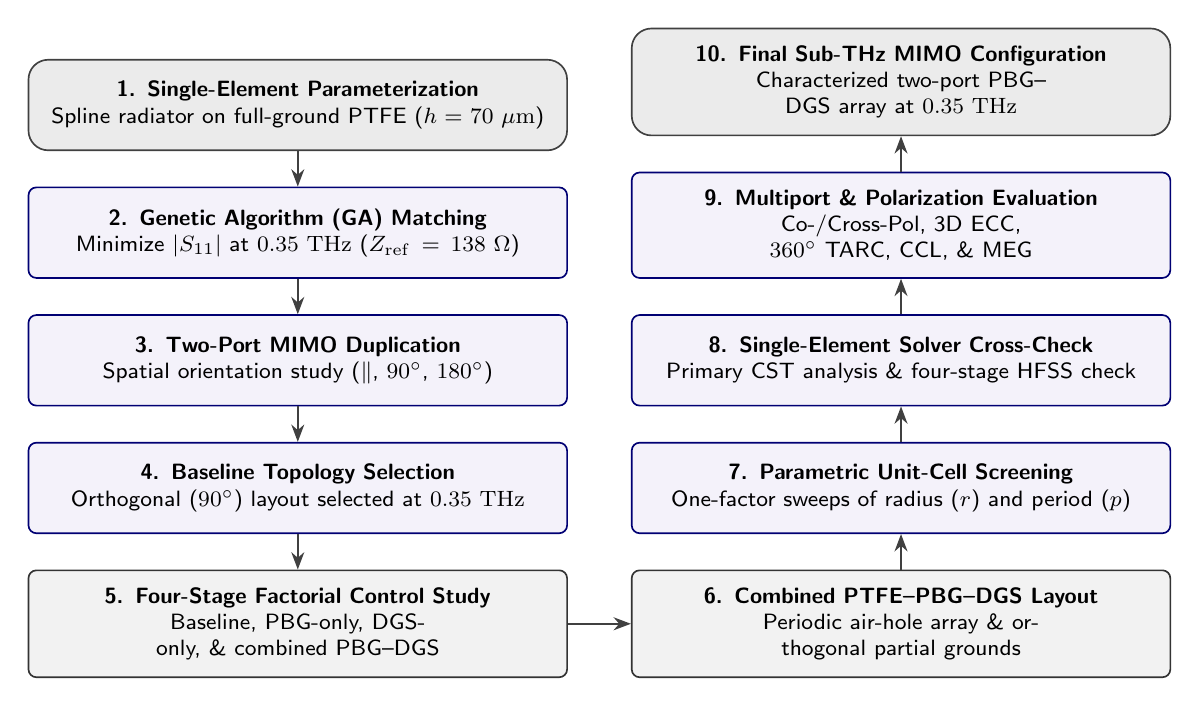
\begin{tikzpicture}[
        node distance=4.5mm and 8mm,
        base/.style={draw, semithick, align=center, inner sep=2.2mm, text width=6.4cm, minimum height=1.15cm, font=\footnotesize\sffamily},
        terminal/.style={base, rectangle, rounded corners=2.5mm, fill=gray!16, draw=black!75},
        process/.style={base, rectangle, rounded corners=1mm, fill=cyan!6!blue!4, draw=blue!45!black},
        highlight/.style={base, rectangle, rounded corners=1mm, fill=gray!10, draw=black!80},
        arrow/.style={-{Stealth[scale=1.1]}, semithick, draw=black!75}
    ]
    % Left Column (Steps 1 to 5)
    \node (n1) [terminal] {\textbf{1. Single-Element Parameterization}\\Spline radiator on full-ground PTFE ($h=70~\mu\mathrm{m}$)};
    \node (n2) [process, below=of n1] {\textbf{2. Genetic Algorithm (GA) Matching}\\Minimize $|S_{11}|$ at $0.35~\mathrm{THz}$ ($Z_{\mathrm{ref}}=138~\Omega$)};
    \node (n3) [process, below=of n2] {\textbf{3. Two-Port MIMO Duplication}\\Spatial orientation study ($\parallel$, $90^\circ$, $180^\circ$)};
    \node (n4) [process, below=of n3] {\textbf{4. Baseline Topology Selection}\\Orthogonal ($90^\circ$) layout selected at $0.35~\mathrm{THz}$};
    \node (n5) [highlight, below=of n4] {\textbf{5. Four-Stage Factorial Control Study}\\Baseline, PBG-only, DGS-only, \& combined PBG--DGS};

    % Right Column (Steps 6 to 10)
    \node (n6) [highlight, right=of n5] {\textbf{6. Combined PTFE--PBG--DGS Layout}\\Periodic air-hole array \& orthogonal partial grounds};
    \node (n7) [process, above=of n6] {\textbf{7. Parametric Unit-Cell Screening}\\One-factor sweeps of radius ($r$) and period ($p$)};
    \node (n8) [process, above=of n7] {\textbf{8. Single-Element Solver Cross-Check}\\Primary CST analysis \& four-stage HFSS check};
    \node (n9) [process, above=of n8] {\textbf{9. Multiport \& Polarization Evaluation}\\Co-/Cross-Pol, 3D ECC, $360^\circ$ TARC, CCL, \& MEG};
    \node (n10) [terminal, above=of n9] {\textbf{10. Final Sub-THz MIMO Configuration}\\Characterized two-port PBG--DGS array at $0.35~\mathrm{THz}$};

    % Connections
    \draw [arrow] (n1) -- (n2);
    \draw [arrow] (n2) -- (n3);
    \draw [arrow] (n3) -- (n4);
    \draw [arrow] (n4) -- (n5);
    \draw [arrow] (n5.east) -- (n6.west);
    \draw [arrow] (n6) -- (n7);
    \draw [arrow] (n7) -- (n8);
    \draw [arrow] (n8) -- (n9);
    \draw [arrow] (n9) -- (n10);
    \end{tikzpicture}
    \caption{Flowchart of the design and evaluation methodology, progressing from single-element spline parameterization (Step~1) and four-stage factorial control analysis (Steps~5--8) to two-port MIMO characterization (Steps~9--10).}
    \label{fig:flowchart}
\end{figure}


% 2.1 Single-Element Geometry and Genetic-Algorithm Optimization

\subsection{Single-Element Geometry and Genetic-Algorithm Optimization}
\label{subsec:single_element_design}

The proposed two-port MIMO antenna is developed from a single planar radiating element, following the ten-step workflow shown in Figure~\ref{fig:flowchart}. In its baseline configuration, the single element is printed on the top surface of a homogeneous dielectric substrate backed by a continuous rectangular ground plane covering the entire bottom surface ($L \times W$). Instead of a canonical rectangular or circular patch, the radiator perimeter is defined by a smooth spline-based contour, which provides geometric flexibility to adjust the effective current path and achieve impedance matching at the target sub-THz frequency while inherently supporting wide-bandwidth operation \citep{marouf_bezier_2023, Bekasiewicz2021, Prasetyo2023ISAP, Prasetyo2023PIERS}.

To halve the number of optimization variables and enforce a symmetric broadside radiation pattern, mirror symmetry is imposed across the central vertical plane ($x=0$, with the microstrip feed line aligned along the $y$-axis). The closed radiator boundary is constructed from an eight-vertex control polygon ($\mathbf{P}_0, \mathbf{P}_1, \dots, \mathbf{P}_7$, with $\mathbf{P}_8 \equiv \mathbf{P}_0$) using a $C^{1}$-continuous, closed piecewise quadratic B\'ezier spline (uniform quadratic B-spline). Specifically, defining the control-polygon edge midpoints as on-curve segment endpoints (knots):
\begin{equation}
\mathbf{M}_k = \frac{\mathbf{P}_k + \mathbf{P}_{(k+1)\bmod 8}}{2}, \qquad k \in \{0, 1, \dots, 7\},
\label{eq:spline_midpoints}
\end{equation}
each of the eight quadratic B\'ezier segments $\mathbf{B}_k(t)$ is uniquely defined over $t \in [0, 1]$ by the control triplet $(\mathbf{M}_{(k-1)\bmod 8}, \mathbf{P}_k, \mathbf{M}_k)$:
\begin{equation}
\mathbf{B}_k(t) = (1-t)^{2}\mathbf{M}_{(k-1)\bmod 8} + 2t(1-t)\mathbf{P}_k + t^{2}\mathbf{M}_k, \qquad t \in [0, 1], \quad k \in \{0, 1, \dots, 7\}.
\label{eq:bezier_segment}
\end{equation}
This construction guarantees closure ($\mathbf{B}_7(1) = \mathbf{M}_7 = \mathbf{B}_0(0)$) and continuous first derivatives ($\mathbf{B}'_k(1) = \mathbf{B}'_{(k+1)\bmod 8}(0) = \mathbf{P}_{(k+1)\bmod 8} - \mathbf{P}_k$) at every junction $\mathbf{M}_k$.

The lower feed-transition apex $\mathbf{P}_0 = (0, 0)$ (where the radiator connects to the upper end of the microstrip feed line of length $L_f = 105~\mu\mathrm{m}$ and width $W_f = 25~\mu\mathrm{m}$) and the upper axial apex $\mathbf{P}_4 = (0, 300~\mu\mathrm{m})$ are fixed on the symmetry axis. The independent coordinates of the three movable right-hand control points ($\mathbf{P}_1, \mathbf{P}_2$, and $\mathbf{P}_3$) form the six-dimensional design vector:
\begin{equation}
\mathbf{x}= \left[ x_1, y_1, x_2, y_2, x_3, y_3 \right]^{T},
\label{eq:design_vector}
\end{equation}
while the left-hand points ($\mathbf{P}_5, \mathbf{P}_6, \mathbf{P}_7$) are enforced by mirror symmetry as $\mathbf{P}_{8-i}=(-x_i,y_i)$ for $i\in\{1,2,3\}$. Each coordinate in $\mathbf{x}$ is constrained within a $\pm10\%$ local search window around its nominal position.

The antenna is modeled on a non-dispersive polytetrafluoroethylene (PTFE) substrate ($\varepsilon_r = 2.7$, $\tan \delta = 0.0002$) with single-element planar dimensions of $L = 625.5~\mu\mathrm{m}$ ($0.73\lambda_0$ at $f_0 = 0.35~\mathrm{THz}$, where $\lambda_0 \approx 857.1~\mu\mathrm{m}$) and $W = 626.25~\mu\mathrm{m}$ ($0.73\lambda_0$), and a thickness of $h = 70.0~\mu\mathrm{m}$ ($0.082\lambda_0$). All metallic layers (radiator, microstrip feed, and ground plane) are modeled using lossy annealed gold from the CST material library ($\sigma = 4.561 \times 10^{7}~\mathrm{S/m}$, smooth conductor surfaces without surface-roughness correction). The microstrip feed dimensions ($W_f = 25~\mu\mathrm{m}$, $L_f = 105~\mu\mathrm{m}$) are kept fixed throughout to isolate the effect of the spline contour and substrate modifications. In CST Microwave Studio, both the single-element and two-port models are excited via single-mode waveguide ports with a zero reference-plane offset at the substrate edge. All reported S-parameters, bandwidths, and active reflection metrics are normalized to the fixed port reference impedance $Z_{\mathrm{ref}}=138~\Omega$, which corresponds to the quasi-TEM characteristic mode impedance of the narrow $25~\mu\mathrm{m}$-wide microstrip line on the $70~\mu\mathrm{m}$ PTFE substrate ($W_f/h = 0.357$).

To tune the radiator contour for input matching at the target frequency $f_0 = 0.35~\mathrm{THz}$, an island-model Genetic Algorithm (GA) in CST (population size 32, partitioned into 4 subpopulations of 8 individuals) was employed to minimize the single-frequency reflection-coefficient magnitude in decibels \citep{Goudos2016}:
\begin{equation}
\min_{\mathbf{x}} J(\mathbf{x}) = 20\log_{10}\left|S_{11}(f_0;\mathbf{x})\right|.
\label{eq:ga_objective}
\end{equation}
Because Eq.~(\ref{eq:ga_objective}) evaluates matching at a single frequency ($f_0 = 0.35~\mathrm{THz}$), the GA serves strictly as a local contour-matching tool rather than a multi-frequency bandwidth optimizer. Table~\ref{tab:ga-settings} and Table~\ref{tab:spline_points} list the GA settings and the retained control-point coordinates, respectively, while Figure~\ref{fig:single_element_geometry} illustrates the single-element geometry.

\begin{table}[ht]
\caption{Configuration parameters of the Genetic Algorithm used for single-frequency contour matching at $f_0 = 0.35~\mathrm{THz}$.}
\label{tab:ga-settings}
\centering
\begin{tabular}{ll}
\hline
\textbf{Parameter} & \textbf{Setting} \\
\hline
Design variables & 6 ($x_1, y_1, x_2, y_2, x_3, y_3$) \\
Search space bounds & $\pm10\%$ around nominal coordinates \\
Population size & 32 (4 subpopulations of 8 individuals) \\
Maximum iterations & 30 \\
Maximum solver evaluations & 497 \\
Mutation rate & 60\% \\
\hline
\end{tabular}
\end{table}

\begin{table}[ht]
\caption{Coordinates of the symmetric piecewise quadratic B\'ezier radiator (in $\mu\mathrm{m}$, relative to $\mathbf{P}_0$ at the feed-line junction). Points $\mathbf{P}_5$, $\mathbf{P}_6$, and $\mathbf{P}_7$ are defined by mirror symmetry $\mathbf{P}_{8-i} = (-x_i, y_i)$; $\mathbf{P}_0$ and $\mathbf{P}_4$ are fixed.}
\label{tab:spline_points}
\centering
\begin{tabular}{lcc}
\hline
\textbf{Point} & \textbf{\(x\)-coordinate (\(\mu\mathrm{m}\))} & \textbf{\(y\)-coordinate (\(\mu\mathrm{m}\))} \\
\hline
\(\mathbf{P}_0\) (fixed) & 0 & 0 \\
\(\mathbf{P}_1\) (tuned) & 90 & 120 \\
\(\mathbf{P}_2\) (tuned) & 180 & 210 \\
\(\mathbf{P}_3\) (tuned) & 260 & 260 \\
\(\mathbf{P}_4\) (fixed) & 0 & 300 \\
\hline
\end{tabular}
\end{table}

\begin{figure}[ht]
    \centering
    \includegraphics[width=0.8\columnwidth]{figures/figure_01.pdf}
    \caption{Geometry of the proposed spline-profiled single antenna element (feed width $W_f$ and length $L_f$). The radiator boundary is defined by independent control points on one side of the symmetry axis ($x=0$), with the opposing points obtained via mirror symmetry.}
    \label{fig:single_element_geometry}
\end{figure}


% 2.2 Two-Port MIMO Configuration and Coupling Analysis

\subsection{Two-Port MIMO Configuration, Spacing Rules, and Active Matching Formulation}
\label{subsec:two_port_mimo}

To construct the two-port sub-THz MIMO configuration, the single-element cell is duplicated side-by-side along the $x$-axis onto a shared PTFE substrate of overall width $W_{\mathrm{MIMO}} = 1252.5~\mu\mathrm{m}$ ($1.46\lambda_0$, comprising two $626.25~\mu\mathrm{m}$-wide half-cells) and length $L_{\mathrm{MIMO}} = 625.5~\mu\mathrm{m}$ ($0.73\lambda_0$). Each radiator is fed by an independent microstrip line ($W_f = 25~\mu\mathrm{m}$, $L_f = 105~\mu\mathrm{m}$) excited by a zero-offset waveguide port normalized to \(Z_{\mathrm{ref}}=138~\Omega\); during single-port excitation, the inactive port is terminated in a matched \(138~\Omega\) load \citep{MIMOReview2022}.

Three candidate relative orientations were evaluated on the homogeneous full-ground PTFE substrate by rotating the second element (Port~2) while maintaining a constant radiator center-to-center pitch of $d_{\mathrm{cc}} = 630.0~\mu\mathrm{m}$ ($0.735\lambda_0$, corresponding to a $1.875~\mu\mathrm{m}$ outward offset from each half-cell midpoint), as shown in Figure~\ref{fig:mimo_orientations} \citep{OrientationStudy2023, taher2023, MIMOOrientationComparison2022}:
\begin{enumerate}
    \item \textbf{Parallel (\(\parallel\), \(0^{\circ}\)) [Figure~\ref{fig:mimo_orientations}(a)]:} Both elements are fed from the bottom substrate edge ($y=0$). Because each spline radiator has a transverse width of $2x_3 = 520.0~\mu\mathrm{m}$ along $x$, the resulting edge-to-edge clearance between the two patches is $d_{\mathrm{e,\parallel}} = d_{\mathrm{cc}} - 520.0~\mu\mathrm{m} = 110.0~\mu\mathrm{m}$ ($0.128\lambda_0$).
    \item \textbf{Orthogonal (\(90^{\circ}\)) [Figure~\ref{fig:mimo_orientations}(b)]:} Port~1 is fed from the bottom edge ($y=0$), whereas Port~2 is rotated by $90^{\circ}$ and fed from the right-hand substrate edge ($x = W_{\mathrm{MIMO}}$). Because Port~2's axial length ($300.0~\mu\mathrm{m}$) now lies along $x$, rotating Port~2 about the same center-to-center pitch ($d_{\mathrm{cc}} = 630.0~\mu\mathrm{m}$) increases the inter-radiator edge-to-edge clearance to $d_{\mathrm{e,90^{\circ}}} = 391.2~\mu\mathrm{m}$ ($0.46\lambda_0$) and separates the feeding ports onto orthogonal substrate edges.
    \item \textbf{Face-to-Face (\(180^{\circ}\)) [Figure~\ref{fig:mimo_orientations}(c)]:} Port~1 is fed from the bottom edge ($y=0$) and Port~2 is rotated by $180^{\circ}$ and fed from the top edge ($y = L_{\mathrm{MIMO}}$), maintaining the same center-to-center pitch $d_{\mathrm{cc}} = 630.0~\mu\mathrm{m}$ and transverse edge-to-edge clearance $d_{\mathrm{e,180^{\circ}}} = 110.0~\mu\mathrm{m}$ ($0.128\lambda_0$).
\end{enumerate}
Based on the simulated coupling response at the target frequency $f_0 = 0.35~\mathrm{THz}$, the orthogonal ($90^{\circ}$) arrangement was selected as the baseline two-port topology for the four-stage substrate and ground-modification study.

Under simultaneous two-port excitation, active impedance matching is evaluated from the full-wave two-port S-matrix (referenced to $Z_{\mathrm{ref}} = 138~\Omega$) using the total active reflection coefficient (TARC) \citep{MIMOReview2022}. For equal-amplitude incident power waves \(a_1=A\) and \(a_2=Ae^{j\Delta\phi}\) (where \(\Delta\phi \in [0^{\circ}, 360^{\circ})\) is the excitation phase offset at Port~2 relative to Port~1), the reflected waves are \(b_1=S_{11}a_1+S_{12}a_2\) and \(b_2=S_{21}a_1+S_{22}a_2\), yielding:
\begin{equation}
\begin{aligned}
\mathrm{TARC}(f,\Delta\phi)
&=\sqrt{\frac{
|S_{11}+S_{12}e^{j\Delta\phi}|^{2}
+|S_{21}+S_{22}e^{j\Delta\phi}|^{2}}{2}},\\
\mathrm{TARC}_{\mathrm{dB}}(f,\Delta\phi)
&=20\log_{10}\!\left(\mathrm{TARC}(f,\Delta\phi)\right).
\end{aligned}
\label{eq:tarc}
\end{equation}
Because an asymmetric two-port network ($S_{11} \neq S_{22}$) is $360^{\circ}$-periodic in $\Delta\phi$, TARC can attain its extremum anywhere over $\Delta\phi \in [0^{\circ}, 360^{\circ})$. Expanding Eq.~(\ref{eq:tarc}) as $\mathrm{TARC}^{2}(f,\Delta\phi) = 0.5(|S_{11}|^{2} + |S_{12}|^{2} + |S_{21}|^{2} + |S_{22}|^{2}) + \mathrm{Re}\{(S_{11}^{*}S_{12} + S_{21}^{*}S_{22})e^{j\Delta\phi}\}$ yields the exact analytical full-cycle ($0^{\circ}$--$360^{\circ}$) worst-case active reflection envelope:
\begin{equation}
\mathrm{TARC}_{\mathrm{worst}}(f) = \max_{\Delta\phi \in [0^{\circ}, 360^{\circ})} \mathrm{TARC}(f, \Delta\phi) = \sqrt{\frac{|S_{11}|^{2}+|S_{12}|^{2}+|S_{21}|^{2}+|S_{22}|^{2}}{2} + \left|S_{11}^{*}S_{12} + S_{21}^{*}S_{22}\right|}.
\label{eq:tarc_worst}
\end{equation}
In Section~\ref{sec:results}, TARC is reported both for five discrete phase offsets ($\Delta\phi = 0^{\circ}, 45^{\circ}, 90^{\circ}, 135^{\circ}, 180^{\circ}$) and for the continuous full-cycle worst-case envelope $\mathrm{TARC}_{\mathrm{worst}}(f)$.

\begin{figure}[!t]
    \centering
    \includegraphics[width=\columnwidth]{figures/figure_02.pdf}
    \caption{Three candidate two-port MIMO layouts on the shared homogeneous PTFE substrate: (a) parallel (\(\parallel\), $0^{\circ}$, top), (b) orthogonal ($90^{\circ}$, middle), and (c) face-to-face ($180^{\circ}$, bottom).}
    \label{fig:mimo_orientations}
\end{figure}


% 2.3 PTFE--PBG--DGS Substrate: Design and Parametric Study

\subsection{Four-Stage PTFE--PBG--DGS Geometry, Parametric Screening, and Solver Cross-Check}
\label{subsec:ptfe_pbg_design}
\label{subsec:single_element_validation}

To systematically separate the electromagnetic effects of dielectric perforation and ground-plane truncation from their combined interaction, both the standalone single element and the orthogonal ($90^{\circ}$) two-port MIMO configuration are evaluated across a four-stage ($2 \times 2$ factorial) sequence \citep{gonzalo1999pbg, coccioli1999ucpbg, zaidi2018pbg, jha2012thz}:
\begin{enumerate}
    \item \textbf{Stage~1 (Homogeneous Baseline):} Unperforated PTFE substrate ($h = 70.0~\mu\mathrm{m}$) backed by a full ground plane ($625.5 \times 626.25~\mu\mathrm{m}^2$ for the single element; $625.5 \times 1252.5~\mu\mathrm{m}^2$ for the two-port layout).
    \item \textbf{Stage~2 (PBG-Only):} A periodic square lattice of cylindrical air holes (radius $r$, center-to-center period $p$, drilled through the full substrate thickness $h = 70.0~\mu\mathrm{m}$) is introduced into the PTFE dielectric while retaining the full ground plane. For the single-element cell, the lattice is arranged on a centered $N_x \times N_y = 5 \times 5$ grid (with outermost hole centers located at $\pm 2p = \pm 246.8~\mu\mathrm{m}$ from the cell center along $x$ and $y$); any hole intersecting the metallic radiator contour or microstrip feed line within a minimum edge-to-edge clearance of $g_{\mathrm{PBG}} = 22.3~\mu\mathrm{m}$ is excluded (i.e., air cylinders are Boolean-subtracted only outside the clearance boundary), as shown in Figure~\ref{fig:pbg_unit_cell}(a).
    \item \textbf{Stage~3 (DGS-Only):} Unperforated homogeneous PTFE substrate combined with a truncated partial rectangular ground plane (defected ground structure, DGS) of length $L_{\mathrm{g}} = 450.5~\mu\mathrm{m}$ along the feed axis, corresponding to an ungrounded truncation window of $\Delta L_{\mathrm{g}} = L - L_{\mathrm{g}} = 625.5 - 450.5 = 175.0~\mu\mathrm{m}$ behind the upper radiator apex, as shown in Figure~\ref{fig:pbg_unit_cell}(b).
    \item \textbf{Stage~4 (Combined PBG--DGS):} Combines the periodic cylindrical air-hole perforation of Stage~2 with the truncated DGS partial ground plane ($L_{\mathrm{g}} = 450.5~\mu\mathrm{m}$, $\Delta L_{\mathrm{g}} = 175.0~\mu\mathrm{m}$) of Stage~3.
\end{enumerate}

At $f_0 = 0.35~\mathrm{THz}$ ($\lambda_0 \approx 857.1~\mu\mathrm{m}$), the guided wavelength estimated from the bulk PTFE permittivity is \(\lambda_g = \lambda_0/\sqrt{\varepsilon_r} \approx 522~\mu\mathrm{m}\). To align the single-element reflection minimum with the $0.35~\mathrm{THz}$ target frequency in the combined PBG--DGS configuration (Stage~4), one-factor-at-a-time parametric screening sweeps were conducted for the air-hole radius ($r = 24, 26, 26.45, 27$, and $28~\mu\mathrm{m}$) and the lattice period ($p = 115, 119, 123.4, 127$, and $131~\mu\mathrm{m}$). The retained period $p = 123.4~\mu\mathrm{m}$ ($p \approx 0.24\,\lambda_g$) and radius $r = 26.45~\mu\mathrm{m}$ ($r/p \approx 0.21$) are summarized in Table~\ref{tab:pbg-params}. Note that while we retain the conventional PBG nomenclature used in the THz patch-antenna literature \citep{khezzar_pbg_2021,babaahmed_hybrid_2025,bouzid_pbg_2025}, the present study evaluates the finite air-hole array empirically via full-wave port and radiation responses rather than claiming an eigenmode dispersion stopband.

To check solver consistency on the elementary radiator, the reflection responses ($|S_{11}|$) of all four single-element stages (Baseline, PBG-only, DGS-only, and PBG--DGS) were simulated in CST Microwave Studio (Finite Integration Technique) and qualitatively cross-checked in ANSYS HFSS (Finite Element Method) \citep{algburi2026csthfss}. All quantitative single-element and two-port MIMO metrics reported in this paper are extracted from CST.

\begin{table}[ht]
\caption{Nominal geometrical parameters of the single-element PTFE--PBG--DGS structure.}
\label{tab:pbg-params}
\centering
\begin{tabular}{llc}
\hline
\textbf{Parameter} & \textbf{Symbol} & \textbf{Value} \\
\hline
Lattice periodicity & \(p\) & 123.4~\(\mu\mathrm{m}\) (\(0.24\lambda_g\)) \\
Air-hole radius & \(r\) & 26.45~\(\mu\mathrm{m}\) (\(r/p = 0.21\)) \\
Substrate thickness & \(h\) & 70.0~\(\mu\mathrm{m}\) (\(0.082\lambda_0\)) \\
Radiator-to-hole minimum clearance & \(g_{\mathrm{PBG}}\) & 22.3~\(\mu\mathrm{m}\) \\
Partial ground-plane length (DGS) & \(L_{\mathrm{g}}\) & 450.5~\(\mu\mathrm{m}\) (\(0.53\lambda_0\)) \\
Ground-plane truncation width & \(\Delta L_{\mathrm{g}}\) & 175.0~\(\mu\mathrm{m}\) (\(0.20\lambda_0\)) \\
Lattice grid (single-element cell) & \(N_x \times N_y\) & \(5 \times 5\) \\
\hline
\end{tabular}
\end{table}

\begin{figure}[ht]
    \centering
    \includegraphics[width=0.85\columnwidth]{figures/figure_03.pdf}
    \caption{Single-element PTFE--PBG--DGS geometry: (a) top view with lattice period \(p\) and air-hole radius \(r\); (b) bottom view showing the truncated partial ground plane (DGS) of length $L_{\mathrm{g}} = 450.5~\mu\mathrm{m}$.}
    \label{fig:pbg_unit_cell}
\end{figure}


% 2.4 Two-Port MIMO with the Combined PBG--DGS Substrate

\subsection{Two-Port Orthogonal MIMO Layout with Combined PBG--DGS Modification}
\label{subsec:mimo_pbg}

In the two-port orthogonal ($90^{\circ}$) MIMO configuration, the $5 \times 5$ unit-cell lattice is replicated across both adjacent half-cells to form a uniform $N_x \times N_y = 10 \times 5$ periodic perforation grid over the shared $1252.5 \times 625.5~\mu\mathrm{m}^2$ PTFE substrate, as detailed in Table~\ref{tab:mimo-params} and illustrated in Figure~\ref{fig:mimo_final_geometry}.

As shown in the bottom view on the right side of Figure~\ref{fig:mimo_final_geometry}, the DGS ground truncation is applied consistently in each port's local coordinate frame: beneath Port~1 (left half-cell, fed along $+y$ from the bottom edge), the ground plane spans $L_{\mathrm{g}} = 450.5~\mu\mathrm{m}$ from the bottom edge ($y \in [0, 450.5~\mu\mathrm{m}]$), leaving a $\Delta L_{\mathrm{g}} = 175.0~\mu\mathrm{m}$ ungrounded window along the top edge ($y \in [450.5, 625.5~\mu\mathrm{m}]$); beneath the $90^{\circ}$-rotated Port~2 (right half-cell, fed along $-x$ from the right edge), the partial ground plane is correspondingly rotated by $90^{\circ}$ so that it extends $L_{\mathrm{g}} = 450.5~\mu\mathrm{m}$ inward from the right-hand feed edge across the full $625.5~\mu\mathrm{m}$ substrate length, leaving a $\Delta L_{\mathrm{g}} = 175.0~\mu\mathrm{m}$ ungrounded strip between the two half-cells.

\begin{table}[ht]
\caption{Geometrical parameters of the two-port orthogonal MIMO layout
($f_0 = 0.35~\mathrm{THz}$, $\lambda_0 = 857.1~\mu\mathrm{m}$, PTFE $h = 70.0~\mu\mathrm{m}$).}
\label{tab:mimo-params}
\centering
\begin{tabular}{llc}
\hline
\textbf{Parameter} & \textbf{Symbol} & \textbf{Value (Electrical Size)} \\
\hline
Edge-to-edge element separation (orthogonal $90^{\circ}$) & \(d_{\mathrm{e}}\)  & 391.2~\(\mu\mathrm{m}\) (\(0.46\lambda_0\)) \\
Edge-to-edge element separation ($\parallel$ and $180^{\circ}$) & \(d_{\mathrm{e,\parallel}}\) & 110.0~\(\mu\mathrm{m}\) (\(0.128\lambda_0\)) \\
Radiator center-to-center pitch (all layouts) & \(d_{\mathrm{cc}}\) & 630.0~\(\mu\mathrm{m}\) (\(0.735\lambda_0\)) \\
Shared substrate width ($2 \times 626.25~\mu\mathrm{m}$) & \(W_{\mathrm{MIMO}}\) & 1252.5~\(\mu\mathrm{m}\) (\(1.46\lambda_0\)) \\
Shared substrate length & \(L_{\mathrm{MIMO}}\) & 625.5~\(\mu\mathrm{m}\) (\(0.73\lambda_0\)) \\
Partial ground-plane length (along each port feed axis) & \(L_{\mathrm{g}}\) & 450.5~\(\mu\mathrm{m}\) (\(0.53\lambda_0\)) \\
Ground-plane truncation width ($L_{\mathrm{MIMO}} - L_{\mathrm{g}}$) & \(\Delta L_{\mathrm{g}}\) & 175.0~\(\mu\mathrm{m}\) (\(0.20\lambda_0\)) \\
Periodic perforation grid (MIMO, total) & \(N_x \times N_y\) & \(10 \times 5\) \\
\hline
\end{tabular}
\end{table}

\begin{figure}[!t]
    \centering
    \includegraphics[width=\columnwidth]{figures/figure_04.pdf}
    \caption{Geometry of the proposed two-port orthogonal MIMO antenna with combined PBG--DGS modification: left, top view showing the spline radiators, $10 \times 5$ air-hole grid, edge-to-edge separation \(d_{\mathrm{e}}\), and overall dimensions \(L_{\mathrm{MIMO}} \times W_{\mathrm{MIMO}}\); right, bottom view showing the orthogonally oriented partial ground planes of length \(L_{\mathrm{g}} = 450.5~\mu\mathrm{m}\) ($\Delta L_{\mathrm{g}} = 175.0~\mu\mathrm{m}$ truncation) beneath Port~1 and Port~2.}
    \label{fig:mimo_final_geometry}
\end{figure}


% 2.5 First-Order Equivalent-Circuit Estimate

\subsection{Local Design-Frequency Series-RLC Estimate for the Baseline Element}
\label{subsec:matching}

To provide a simple lumped-element representation of the port input impedance at the target design frequency $f_0 = 0.350~\mathrm{THz}$, a local first-order series \(R\)--\(L\)--\(C\) network is defined at the zero-offset CST waveguide-port reference plane for the homogeneous-PTFE single-element baseline (Figure~\ref{fig:baseline_rlc_model}):
\begin{equation}
R_{\mathrm{in}} \approx 137~\Omega, \qquad
L_{\mathrm{in}} \approx 79~\mathrm{pH}, \qquad
C_{\mathrm{in}} \approx 3.0~\mathrm{fF}.
\label{eq:rlc}
\end{equation}
Because the CST baseline reflection minimum occurs at $0.3424~\mathrm{THz}$, the antenna exhibits a slightly inductive input impedance ($Z_{11} \approx 128.9 + j21.9~\Omega$) at $0.350~\mathrm{THz}$. Accordingly, the series $L_{\mathrm{in}}C_{\mathrm{in}}$ branch in Eq.~(\ref{eq:rlc}) has its zero-reactance point near $0.327~\mathrm{THz}$ so that at $0.350~\mathrm{THz}$ it yields $Z_{\mathrm{in}}(0.350~\mathrm{THz}) \approx 137 + j22.2~\Omega$, matching the complex CST port impedance within approximately $6\%$ at the design frequency. This three-element network serves strictly as a single-frequency local impedance approximation at $0.350~\mathrm{THz}$ rather than a wideband analytical model.

\begin{figure}[ht]
    \centering
    \begin{circuitikz}[font=\footnotesize]
        % --- ground rail ---
        \draw (0,-1.5) -- (6.2,-1.5);
        \node[ground] at (3.1,-1.5) {};

        % --- Port (left) ---
        \draw (0,-1.5) -- (0,0);
        \draw (0,0) to[short, o-] (1.2,0);
        \node[left] at (-0.1,0) {Port (\(Z_{\mathrm{ref}}=138~\Omega\))};

        \draw (1.2,0) to[R, l=\(R_{\mathrm{in}} \approx 137~\Omega\)] (2.8,0);
        \draw (2.8,0) to[L, l=\(L_{\mathrm{in}}\)] (4.2,0);
        \draw (4.2,0) to[C, l=\(C_{\mathrm{in}}\)] (5.6,0);
        \draw (5.6,0) -- (5.6,-1.5);
        \node[above] at (3.4,0.65) {Baseline Element (local $0.35~\mathrm{THz}$ estimate)};
    \end{circuitikz}
    \caption{Local first-order series-RLC circuit estimate of the homogeneous-PTFE single-element baseline at $0.350~\mathrm{THz}$, referenced to the zero-offset CST waveguide port \(Z_{\mathrm{ref}}=138~\Omega\).}
    \label{fig:baseline_rlc_model}
\end{figure}




\section{Results and Analysis}
\label{sec:results}


% SECTION 3.1: Single-Element Baseline Performance on Homogeneous PTFE

\subsection{Single-Element Baseline Performance on Homogeneous PTFE}
\label{subsec:baseline_performance}

The spline-profiled radiator was first characterized on the homogeneous full-ground PTFE substrate (Stage~1) to establish the reference response relative to the zero-offset waveguide port ($Z_{\mathrm{ref}} = 138~\Omega$). Figure~\ref{fig:single_baseline_s11} presents the simulated input reflection coefficient (\(|S_{11}|\)) over $0.30$--$0.50~\mathrm{THz}$ from CST Microwave Studio alongside a qualitative cross-check from ANSYS HFSS. Both solvers place the primary resonance in the $0.34$--$0.35~\mathrm{THz}$ window, with CST predicting a reflection minimum of \(-30.53~\mathrm{dB}\) at \(0.3424~\mathrm{THz}\) and HFSS showing a primary minimum of \(-25.7~\mathrm{dB}\) near \(0.346~\mathrm{THz}\) (accompanied by a secondary upper-band dip near $0.442~\mathrm{THz}$ attributable to differences in port and mesh discretization between the tetrahedral FEM and hexahedral FIT solvers).

In the primary CST simulation, the \(-10~\mathrm{dB}\) impedance band spans from \(f_L=0.3192~\mathrm{THz}\) to \(f_H=0.4266~\mathrm{THz}\) (both band edges visible within the plotted $0.30$--$0.50~\mathrm{THz}$ window of Figure~\ref{fig:single_baseline_s11}), yielding an absolute bandwidth of \(107.47~\mathrm{GHz}\). Referencing fractional bandwidth to the band-edge midpoint \(f_c=(f_H+f_L)/2=0.3729~\mathrm{THz}\) as \(\mathrm{FBW}=100(f_H-f_L)/f_c\), the homogeneous baseline element achieves an FBW of \(28.82\%\). At its $0.34~\mathrm{THz}$ gain peak, the baseline radiator achieves a realized gain of \(7.22~\mathrm{dBi}\) and a total efficiency $\eta_{\mathrm{tot}} = \eta_{\mathrm{rad}}(1 - |S_{11}|^{2})$ of \(95.2\%\) (decreasing to \(7.02~\mathrm{dBi}\) and \(\eta_{\mathrm{tot}} = 93.5\%\) at $0.350~\mathrm{THz}$).

\begin{figure}[ht]
    \centering
    \includegraphics[width=0.85\linewidth]{figures/figure_05.pdf}
    \caption{Simulated reflection coefficient $|S_{11}|$ ($Z_{\mathrm{ref}}=138~\Omega$) of the standalone spline-profiled antenna on the homogeneous full-ground PTFE substrate (Stage~1) over $0.30$--$0.50~\mathrm{THz}$, showing both $-10~\mathrm{dB}$ band edges ($0.3192$ and $0.4266~\mathrm{THz}$) in CST alongside a qualitative HFSS check.}
    \label{fig:single_baseline_s11}
\end{figure}


% SECTION 3.2: Two-Port MIMO Coupling Analysis on Homogeneous Substrate

\subsection{Two-Port MIMO Orientation Study on Homogeneous Substrate}
\label{subsec:mimo_coupling}

Before introducing dielectric perforation or ground truncation, the three candidate two-port orientations defined in Section~\ref{subsec:two_port_mimo}---parallel ($\parallel$, $0^{\circ}$, $d_{\mathrm{cc}} = 630.0~\mu\mathrm{m}$, $d_{\mathrm{e}} = 110.0~\mu\mathrm{m}$), orthogonal ($90^{\circ}$, $d_{\mathrm{cc}} = 630.0~\mu\mathrm{m}$, $d_{\mathrm{e}} = 391.2~\mu\mathrm{m}$), and face-to-face ($180^{\circ}$, $d_{\mathrm{cc}} = 630.0~\mu\mathrm{m}$, $d_{\mathrm{e}} = 110.0~\mu\mathrm{m}$)---were compared on the shared homogeneous full-ground PTFE substrate.

Figure~\ref{fig:mimo_coupling_s21} reports the simulated mutual coupling (\(|S_{21}|\)) over \(0.30\)--\(0.40~\mathrm{THz}\). The parallel layout exhibits the strongest inter-port transmission, peaking at \(-16.98~\mathrm{dB}\) ($0.375~\mathrm{THz}$) with \(|S_{21}| = -18.58~\mathrm{dB}\) at \(0.350~\mathrm{THz}\). Rotating Port~2 by \(180^{\circ}\) (face-to-face, moving the second feed port to the opposite substrate edge while keeping $d_{\mathrm{e}} = 110.0~\mu\mathrm{m}$) reduces \(|S_{21}|\) at \(0.350~\mathrm{THz}\) to \(-20.0~\mathrm{dB}\) and produces a localized transmission dip near \(0.375~\mathrm{THz}\), outside the primary $0.35~\mathrm{THz}$ target window \citep{OrientationStudy2023,taher2023}. At the target frequency of \(0.350~\mathrm{THz}\), the orthogonal (\(90^{\circ}\)) layout yields the lowest inter-port transmission among the three tested geometries, with \(|S_{21}|\approx-23.5~\mathrm{dB}\). As noted in Section~\ref{subsec:two_port_mimo}, this $-23.5~\mathrm{dB}$ baseline level reflects the combined benefit of orthogonal polarization, wider edge-to-edge clearance ($391.2~\mu\mathrm{m}$), and orthogonal feed placement.

Figure~\ref{fig:current_homogeneous} illustrates the scalar surface-current magnitude distribution of the orthogonal homogeneous baseline (Stage~1) at \(0.35~\mathrm{THz}\) with Port~1 excited and Port~2 matched to \(Z_{\mathrm{ref}} = 138~\Omega\), showing residual current coupled onto the passive Port~2 radiator and feed line.

\begin{figure}[ht]
    \centering
    \includegraphics[width=0.85\linewidth]{figures/figure_06.pdf}
    \caption{Simulated mutual coupling \(|S_{21}|\) ($Z_{\mathrm{ref}} = 138~\Omega$) of the two-port MIMO antenna on a homogeneous full-ground PTFE substrate for the parallel (\(\parallel\), $0^{\circ}$), face-to-face (\(180^{\circ}\)), and orthogonal (\(90^{\circ}\)) layouts.}
    \label{fig:mimo_coupling_s21}
\end{figure}

\begin{figure}[ht]
    \centering
    \includegraphics[width=0.85\linewidth]{figures/figure_07.pdf}
    \caption{Simulated scalar surface-current magnitude distribution of the orthogonal ($90^{\circ}$) configuration on the homogeneous full-ground PTFE substrate (Stage~1) at \(0.35~\mathrm{THz}\), with Port~1 excited and Port~2 matched to \(Z_{\mathrm{ref}} = 138~\Omega\).}
    \label{fig:current_homogeneous}
\end{figure}


% SECTION 3.3: Performance of the Single Element with PBG and DGS Integration

\subsection{Single-Element Parametric Screening and Four-Stage Control Analysis}
\label{subsec:single_pbg_performance}

To align the single-element reflection minimum with the \(0.35~\mathrm{THz}\) target frequency in the combined PBG--DGS configuration (Stage~4, incorporating both the perforated substrate and the truncated ground plane of length \(L_{\mathrm{g}} = 450.5~\mu\mathrm{m}\)), one-factor-at-a-time parametric screening sweeps were conducted for the air-hole radius (\(r = 24, 26, 26.45, 27\), and \(28~\mu\mathrm{m}\) at fixed \(p = 123.4~\mu\mathrm{m}\)) and the lattice period (\(p = 115, 119, 123.4, 127\), and \(131~\mu\mathrm{m}\) at fixed \(r = 26.45~\mu\mathrm{m}\)), as shown in Figure~\ref{fig:parametric_p_r}.

As shown in Figure~\ref{fig:parametric_p_r}(a), increasing the air-hole radius \(r\) from \(24~\mu\mathrm{m}\) to \(28~\mu\mathrm{m}\) shifts the resonant frequency of the PBG--DGS radiator monotonically upward from \(0.349~\mathrm{THz}\) (\(|S_{11}| = -34.2~\mathrm{dB}\)) to \(0.354~\mathrm{THz}\) (\(|S_{11}| = -60.3~\mathrm{dB}\)), consistent with the progressive reduction in effective substrate permittivity as a larger dielectric volume fraction is removed \citep{jha2012thz}. While \(r = 28~\mu\mathrm{m}\) produces the deepest notch, its minimum shifts above the \(0.350~\mathrm{THz}\) target; consequently, \(r = 26.45~\mu\mathrm{m}\) (\(|S_{11}| = -43.12~\mathrm{dB}\) at \(0.3517~\mathrm{THz}\)) was retained to balance return-loss depth and target-frequency alignment. Conversely, Figure~\ref{fig:parametric_p_r}(b) shows that varying the lattice period \(p\) primarily modulates the return-loss depth while keeping the resonance centered near \(0.352~\mathrm{THz}\): the reflection minimum deepens from \(-34.7~\mathrm{dB}\) (\(p = 115~\mu\mathrm{m}\)) to \(-43.12~\mathrm{dB}\) at \(p = 123.4~\mu\mathrm{m}\), before shallowing to \(-33.8~\mathrm{dB}\) (\(p = 127~\mu\mathrm{m}\)) and \(-28.9~\mathrm{dB}\) (\(p = 131~\mu\mathrm{m}\)).

\begin{figure}[!t]
    \centering
    \begin{minipage}{0.485\textwidth}
        \centering
        \includegraphics[width=\linewidth]{figures/figure_08.pdf}
        \centerline{(a)}
    \end{minipage}\hfill
    \begin{minipage}{0.485\textwidth}
        \centering
        \includegraphics[width=\linewidth]{figures/figure_09.pdf}
        \centerline{(b)}
    \end{minipage}
    \caption{One-factor-at-a-time parametric screening of the standalone PBG--DGS single-element antenna (Stage~4, $Z_{\mathrm{ref}} = 138~\Omega$): simulated reflection coefficient \(|S_{11}|\) for (a) varying air-hole radius \(r\) (at fixed \(p = 123.4~\mu\mathrm{m}\)) and (b) varying lattice periodicity \(p\) (at fixed \(r = 26.45~\mu\mathrm{m}\)).}
    \label{fig:parametric_p_r}
\end{figure}

Figure~\ref{fig:single_pbg_s11_gain} compares the single-element reflection coefficient (\(|S_{11}|\) over $0.25$--$0.45~\mathrm{THz}$, including qualitative HFSS traces for the three modified stages), realized gain, and total efficiency ($\eta_{\mathrm{tot}}$) across all four factorial stages (Baseline, PBG-only, DGS-only, and Combined PBG--DGS). Examining the individual stages in Figure~\ref{fig:single_pbg_s11_gain} and Table~\ref{tab:four_stage_summary} reveals the distinct empirical role of each modification on the standalone radiator:
\begin{enumerate}
    \item \textbf{DGS-Only (Stage~3 vs.\ Stage~1):} Truncating the ground plane without dielectric perforation shifts the primary CST resonance downward to \(0.3385~\mathrm{THz}\) with a shallower reflection minimum of \(-21.30~\mathrm{dB}\) (\(|S_{11}| = -16.2~\mathrm{dB}\) at $0.350~\mathrm{THz}$; \(-10~\mathrm{dB}\) band from \(0.3175\) to \(0.4385~\mathrm{THz}\), \(\mathrm{FBW} = 32.01\%\)). Moreover, removing the rear ground reflector reduces the $0.350~\mathrm{THz}$ broadside realized gain to \(6.76~\mathrm{dBi}\) ($6.90~\mathrm{dBi}$ at $0.34~\mathrm{THz}$, Figure~\ref{fig:single_pbg_s11_gain}(b)) and lowers the $0.350~\mathrm{THz}$ total efficiency to \(91.2\%\) (Figure~\ref{fig:single_pbg_s11_gain}(c)).
    \item \textbf{PBG-Only (Stage~2 vs.\ Stage~1):} Perforating the PTFE substrate over the full ground plane lowers the effective permittivity, shifting the resonance upward to \(0.3555~\mathrm{THz}\) with a reflection minimum of \(-22.50~\mathrm{dB}\) (\(-10~\mathrm{dB}\) band from \(0.3315\) to \(0.4435~\mathrm{THz}\), \(\mathrm{FBW} = 28.90\%\)), while increasing the $0.350~\mathrm{THz}$ broadside realized gain to \(7.49~\mathrm{dBi}\) and total efficiency to \(95.5\%\).
    \item \textbf{Combined PBG--DGS (Stage~4):} Combining the periodic air-hole array with the truncated DGS ground aligns the resonant minimum at \(0.3517~\mathrm{THz}\) with a deep return loss of \(-43.12~\mathrm{dB}\) (\(-10~\mathrm{dB}\) band from \(0.3302\) to \(0.4483~\mathrm{THz}\), \(f_c = 0.3892~\mathrm{THz}\), \(\mathrm{FBW} = 30.33\%\)). Crucially, introducing the periodic perforation into the DGS-backed element restores the $0.350~\mathrm{THz}$ broadside realized gain from \(6.76~\mathrm{dBi}\) (DGS-only) to \(7.22~\mathrm{dBi}\) and recovers the total efficiency from \(91.2\%\) to \(95.41\%\) (where $\eta_{\mathrm{tot}} \approx \eta_{\mathrm{rad}} = 95.41\%$ near resonance due to negligible mismatch loss, $|S_{11}|^{2} < 10^{-4}$). The qualitative HFSS traces in Figure~\ref{fig:single_pbg_s11_gain}(a) exhibit the same relative frequency ordering across stages, with DGS-only resonating lowest ($\approx 0.331~\mathrm{THz}$) and the perforated configurations shifting upward into the $0.345$--$0.350~\mathrm{THz}$ window.
\end{enumerate}

\begin{figure}[!t]
    \centering
    \begin{minipage}{0.485\textwidth}
        \centering
        \includegraphics[width=\linewidth]{figures/figure_10.pdf}
        \centerline{(a)}
    \end{minipage}\hfill
    \begin{minipage}{0.485\textwidth}
        \centering
        \includegraphics[width=\linewidth]{figures/figure_11.pdf}
        \centerline{(b)}
    \end{minipage}
    \par\medskip
    \begin{minipage}{0.50\textwidth}
        \centering
        \includegraphics[width=\linewidth]{figures/figure_12.pdf}
        \centerline{(c)}
    \end{minipage}
    \caption{Four-stage single-element performance comparison ($Z_{\mathrm{ref}}=138~\Omega$): (a) reflection coefficient \(|S_{11}|\) over $0.25$--$0.45~\mathrm{THz}$ for PBG-only, DGS-only, and combined PBG--DGS in CST and HFSS (baseline shown in Figure~\ref{fig:single_baseline_s11}); (b) CST realized gain (dBi); (c) CST total efficiency ($\eta_{\mathrm{tot}}$).}
    \label{fig:single_pbg_s11_gain}
\end{figure}


% SECTION 3.4: MIMO PERFORMANCE WITH PBG

\subsection{Four-Stage Factorial Control Analysis in the Two-Port MIMO Antenna}
\label{subsec:mimo_pbg_performance}

Following the single-element study, the orthogonal ($90^{\circ}$) two-port MIMO layout was evaluated in CST across the same four factorial stages: Stage~1 (Baseline), Stage~2 (PBG-only), Stage~3 (DGS-only), and Stage~4 (Combined PBG--DGS). Because the orthogonal layout is geometrically asymmetric with respect to the shared substrate boundaries, both port reflection coefficients (\(|S_{11}|\) and \(|S_{22}|\)) are plotted over $0.30$--$0.50~\mathrm{THz}$ in Figure~\ref{fig:mimo_reflection_pbg_dgs}, while the inter-port transmission coefficient (\(|S_{21}|\)) is compared over $0.30$--$0.40~\mathrm{THz}$ in Figure~\ref{fig:mimo_pbg_s21}. All quantitative single-element and two-port metrics across the four stages are summarized in Table~\ref{tab:four_stage_summary}.

\begin{figure}[!t]
    \centering
    \begin{minipage}{0.485\textwidth}
        \centering
        \includegraphics[width=\linewidth]{figures/figure_13.pdf}
        \centerline{(a)}
    \end{minipage}\hfill
    \begin{minipage}{0.485\textwidth}
        \centering
        \includegraphics[width=\linewidth]{figures/figure_14.pdf}
        \centerline{(b)}
    \end{minipage}
    \caption{Simulated two-port reflection coefficients ($Z_{\mathrm{ref}} = 138~\Omega$) over $0.30$--$0.50~\mathrm{THz}$ across all four factorial stages (Baseline, DGS-only, PBG-only, and Combined PBG--DGS): (a) Port~1 \(|S_{11}|\); (b) Port~2 \(|S_{22}|\).}
    \label{fig:mimo_reflection_pbg_dgs}
\end{figure}

\begin{figure}[ht]
    \centering
    \includegraphics[width=0.85\linewidth]{figures/figure_15.pdf}
    \caption{Simulated inter-port transmission coefficient \(|S_{21}|\) ($Z_{\mathrm{ref}} = 138~\Omega$) for the orthogonal ($90^{\circ}$) two-port MIMO antenna across all four factorial stages: Homogeneous Baseline, DGS-only, PBG-only, and Combined PBG--DGS.}
    \label{fig:mimo_pbg_s21}
\end{figure}

Comparing the four two-port stages in Figures~\ref{fig:mimo_reflection_pbg_dgs}--\ref{fig:mimo_pbg_s21} and Table~\ref{tab:four_stage_summary} establishes the specific contribution of each modification:
\begin{enumerate}
    \item \textbf{Effect of Perforation Alone (Stage~2, PBG-Only):} On the full ground plane, introducing the $10 \times 5$ air-hole array shifts the port reflection minima upward from $0.3430 / 0.3405~\mathrm{THz}$ (Baseline) to $0.3563 / 0.3555~\mathrm{THz}$, but produces only a minor change in $|S_{21}|$ across the focused $0.327$--$0.383~\mathrm{THz}$ band ($|S_{21}| = -23.8~\mathrm{dB}$ at $0.350~\mathrm{THz}$ versus $-23.5~\mathrm{dB}$ for the baseline).
    \item \textbf{Effect of Ground Truncation Alone (Stage~3, DGS-Only):} Truncating the ground planes beneath both ports without dielectric perforation substantially reduces inter-port transmission across the lower and central portions of the band, yielding $|S_{21}| = -32.2~\mathrm{dB}$ at $0.350~\mathrm{THz}$ and a transmission dip of $-39.4~\mathrm{dB}$ near $0.368~\mathrm{THz}$ (with $|S_{21}|$ ranging from $-28.9$ to $-39.4~\mathrm{dB}$ over $0.327$--$0.383~\mathrm{THz}$). However, as in the single-element case, DGS-only leaves both ports detuned below the target frequency ($0.3400~\mathrm{THz}$ for Port~1 and $0.3390~\mathrm{THz}$ for Port~2) with shallower reflection minima ($|S_{11}|_{\min} = -23.5~\mathrm{dB}$, $|S_{22}|_{\min} = -23.3~\mathrm{dB}$) and degraded matching at $0.350~\mathrm{THz}$ ($-18.2~\mathrm{dB}$ and $-17.2~\mathrm{dB}$).
    \item \textbf{Combined Effect in the Proposed PBG--DGS Configuration (Stage~4):} The four-stage comparison demonstrates that while the DGS ground truncation is the primary driver of the $\approx 8~\mathrm{dB}$ coupling reduction at $0.350~\mathrm{THz}$ ($|S_{21}| = -31.5~\mathrm{dB}$ for PBG--DGS and $-32.2~\mathrm{dB}$ for DGS-only, compared with $-23.5~\mathrm{dB}$ for the baseline), combining the periodic air-hole perforation with the DGS is essential to simultaneously: (i)~re-center the port resonances onto the target window ($0.3533~\mathrm{THz}$ with $|S_{11}|_{\min} = -43.7~\mathrm{dB}$ at Port~1, and $0.3520~\mathrm{THz}$ with $|S_{22}|_{\min} = -49.3~\mathrm{dB}$ at Port~2, improving $0.350~\mathrm{THz}$ matching by $>10~\mathrm{dB}$ over DGS-only); (ii)~deepen the upper-band transmission notch by an additional $15.8~\mathrm{dB}$, from $-39.4~\mathrm{dB}$ (DGS-only at $0.368~\mathrm{THz}$) to \(-55.2~\mathrm{dB}\) at \(0.3772~\mathrm{THz}\) (maintaining $|S_{21}|$ between $-29.8$ and $-55.2~\mathrm{dB}$ across $0.327$--$0.383~\mathrm{THz}$); and (iii)~recover the broadside gain and total efficiency lost by the DGS truncation. Physically, these empirical trends are consistent with the hypothesis that ground truncation disrupts common-ground return currents while dielectric perforation lowers the effective permittivity to restore impedance matching and reduce residual substrate-mode coupling at higher frequencies.
\end{enumerate}

Figure~\ref{fig:current_pbg} shows the simulated scalar surface-current magnitude map for the combined PBG--DGS two-port configuration at \(0.35~\mathrm{THz}\) under Port~1 excitation, confirming reduced current excitation on the terminated Port~2 structure compared with the homogeneous baseline (Figure~\ref{fig:current_homogeneous}).

\begin{table}[ht]
\caption{Unified four-stage ($2 \times 2$ factorial) CST performance summary for the standalone single element and the orthogonal ($90^{\circ}$) two-port MIMO configuration ($Z_{\mathrm{ref}} = 138~\Omega$). Fractional bandwidth (FBW) is referenced to the midpoint of the $-10~\mathrm{dB}$ band edges ($f_L$--$f_H$).}
\label{tab:four_stage_summary}
\centering
\renewcommand{\arraystretch}{1.2}
\scriptsize
\setlength{\tabcolsep}{3pt}
\begin{tabularx}{\textwidth}{@{}>{\raggedright\arraybackslash}p{2.3cm} C{1.75cm} C{1.85cm} C{2.05cm} C{1.55cm} C{1.65cm} C{1.85cm} >{\centering\arraybackslash}X@{}}
\toprule
\textbf{Stage / Configuration} & \textbf{Single $f_r$ (THz) / Min.\ $|S_{11}|$ (dB)} & \textbf{Single $-10$~dB Band (THz) / FBW} & \textbf{Single Gain (dBi) / $\eta_{\mathrm{tot}}$ (\%) at $0.35$~THz} & \textbf{MIMO $f_{r1}, f_{r2}$ (THz)} & \textbf{MIMO Min.\ $|S_{11}|, |S_{22}|$ (dB)} & \textbf{MIMO $-10$~dB Band Port~1, Port~2 (THz)} & \textbf{MIMO $|S_{21}|$ at $0.35$~THz / Min.\ (dB)} \\
\midrule
\textbf{1.\ Baseline} (Homog.\ + Full Gnd) & $0.3424$ / $-30.53$ & $0.3192$--$0.4266$ ($28.82\%$) & $7.02$ ($7.22^{a}$) / $93.5$ ($95.2^{a}$) & $0.3430$, $0.3405$ & $-24.7$, $-45.0$ & $0.320$--$0.428$, $0.317$--$0.424$ & $-23.5$ / $-24.5$ \\
\textbf{2.\ PBG-Only} (Perforated + Full Gnd) & $0.3555$ / $-22.50$ & $0.3315$--$0.4435$ ($28.90\%$) & $7.49$ / $95.5$ & $0.3563$, $0.3555$ & $-32.7$, $-23.7$ & $0.333$--$0.441$, $0.329$--$0.439$ & $-23.8$ / $-25.8$ \\
\textbf{3.\ DGS-Only} (Homog.\ + Trunc.\ Gnd) & $0.3385$ / $-21.30$ & $0.3175$--$0.4385$ ($32.01\%$) & $6.76$ ($6.90^{a}$) / $91.2$ ($92.7^{a}$) & $0.3400$, $0.3390$ & $-23.5$, $-23.3$ & $0.318$--$0.441$, $0.317$--$0.434$ & $-32.2$ / $-39.4$ \\
\textbf{4.\ PBG--DGS} (Proposed Combined) & $\mathbf{0.3517}$ / $\mathbf{-43.12}$ & $\mathbf{0.3302}$--$\mathbf{0.4483}$ ($\mathbf{30.33\%}$) & $\mathbf{7.22}$ ($7.28^{a}$) / $\mathbf{95.41}$ & $\mathbf{0.3533}$, $\mathbf{0.3520}$ & $\mathbf{-43.7}$, $\mathbf{-49.3}$ & $\mathbf{0.330}$--$\mathbf{0.450}$, $\mathbf{0.329}$--$\mathbf{0.445}$ & $\mathbf{-31.5}$ / $\mathbf{-55.2}$ \\
\bottomrule
\end{tabularx}
\par\smallskip
\begin{minipage}{\textwidth}
\RaggedRight\footnotesize $^{a}$Parenthetical gain and total efficiency values denote the peak at $0.340~\mathrm{THz}$. Two-port in-band minimum $|S_{21}|$ values refer to the focused $0.327$--$0.383~\mathrm{THz}$ interval (occurring at $0.368~\mathrm{THz}$ for DGS-only and $0.3772~\mathrm{THz}$ for Combined PBG--DGS).
\end{minipage}
\end{table}

\begin{figure}[ht]
    \centering
    \includegraphics[width=0.85\linewidth]{figures/figure_16.pdf}
    \caption{Simulated scalar surface-current magnitude distribution for the combined PBG--DGS two-port antenna (Stage~4) at \(0.35~\mathrm{THz}\), with Port~1 excited and Port~2 matched to \(Z_{\mathrm{ref}} = 138~\Omega\).}
    \label{fig:current_pbg}
\end{figure}


% SECTION 3.5: RADIATION & MIMO DIVERSITY METRICS

\subsection{Radiation Characteristics and MIMO Diversity Performance}
\label{subsec:radiation_and_diversity}

The far-field radiation patterns of the combined PBG--DGS two-port antenna (Stage~4) were evaluated at \(0.35~\mathrm{THz}\) over a $1^{\circ} \times 1^{\circ}$ spherical angular grid ($\Delta\theta = 1^{\circ}$, $\Delta\phi = 1^{\circ}$) by exciting one port at a time while terminating the companion port in \(Z_{\mathrm{ref}} = 138~\Omega\). Figure~\ref{fig:farfield_patterns} presents the simulated two-dimensional co-polarization (Co-Pol) and cross-polarization (Cross-Pol) realized-gain polar cuts in the two principal elevation planes (\(\phi=0^{\circ}\) and \(\phi=90^{\circ}\)) for both Port~1 and Port~2.

In each port's local feed-aligned Ludwig-3 coordinate basis, the dominant electric-field component is aligned with its feed axis ($\hat{y}$ for Port~1; $\hat{x}$ for the $90^{\circ}$-rotated Port~2). Equivalently, when referenced to a single common global Ludwig-3 basis (with the reference axis along $\hat{y}$ and the orthogonal axis along $\hat{x}$), Port~1's local Co-Pol and Cross-Pol correspond to the global $\hat{y}$ and $\hat{x}$ components, whereas Port~2's local Co-Pol and Cross-Pol correspond to the global $\hat{x}$ and $\hat{y}$ components, respectively. When Port~1 is excited (Figure~\ref{fig:farfield_patterns}(a)), the antenna radiates a directional broadside beam with a peak Co-Pol ($\hat{y}$) realized gain of \(7.66~\mathrm{dBi}\) and a back-lobe level of \(-12.04~\mathrm{dBi}\) at \(\theta = 180^{\circ}\) (front-to-back ratio of \(19.7~\mathrm{dB}\)). At broadside (\(\theta = 0^{\circ}\)), the Cross-Pol ($\hat{x}$) level is \(-17.32~\mathrm{dBi}\), yielding a broadside cross-polarization discrimination (XPD) of \(24.97~\mathrm{dB}\) (\(\approx 25~\mathrm{dB}\)), while Cross-Pol across the entire \(\phi = 90^{\circ}\) plane remains between \(-15.27~\mathrm{dBi}\) and \(-24.47~\mathrm{dBi}\). Conversely, when Port~2 is excited (Figure~\ref{fig:farfield_patterns}(b)), the principal E- and H-plane cuts interchange, achieving a peak Co-Pol ($\hat{x}$) realized gain of \(7.45~\mathrm{dBi}\) and a broadside Cross-Pol ($\hat{y}$) level of \(-18.80~\mathrm{dBi}\) (\(\mathrm{XPD} = 26.23~\mathrm{dB}\)), with Cross-Pol in the \(\phi = 0^{\circ}\) plane suppressed below \(-11.53~\mathrm{dBi}\) (reaching \(-41.63~\mathrm{dBi}\) at $\theta = 199^{\circ}$ and \(-45.58~\mathrm{dBi}\) in the $\phi = 90^{\circ}$ cut at $\theta = 220^{\circ}$). This complementary $\hat{y}$/$\hat{x}$ polarization behavior in the common global frame is consistent with low far-field pattern correlation.

\begin{figure}[!t]
    \centering
    \begin{minipage}{0.485\textwidth}
        \centering
        \includegraphics[width=\linewidth]{figures/figure_17.pdf}
        \centerline{(a)}
    \end{minipage}\hfill
    \begin{minipage}{0.485\textwidth}
        \centering
        \includegraphics[width=\linewidth]{figures/figure_18.pdf}
        \centerline{(b)}
    \end{minipage}
    \caption{Simulated two-dimensional Ludwig-3 Co-Pol and Cross-Pol far-field realized-gain polar cuts (in dBi, radial scale $-50$ to $10~\mathrm{dBi}$) of the combined PBG--DGS two-port MIMO antenna at \(0.35~\mathrm{THz}\) in the \(\phi=0^{\circ}\) and \(\phi=90^{\circ}\) principal planes: (a) Port~1 excited (local Co-Pol along global $\hat{y}$, Port~2 matched to \(Z_{\mathrm{ref}}\)); (b) Port~2 excited (local Co-Pol along global $\hat{x}$, Port~1 matched to \(Z_{\mathrm{ref}}\)).}
    \label{fig:farfield_patterns}
\end{figure}

To evaluate far-field pattern correlation, the envelope correlation coefficient (\(\mathrm{ECC}_{12}\)) is computed in CST post-processing from the complex three-dimensional embedded far-field electric-field patterns $\mathbf{E}_1(\theta,\phi)$ and $\mathbf{E}_2(\theta,\phi)$ (expressed in a common spherical coordinate basis with $\Delta\theta = \Delta\phi = 1^{\circ}$ quadrature) under the standard assumption of an unweighted, uniform isotropic propagation environment:
\begin{equation}
\mathrm{ECC}_{12}=
\frac{\left|\displaystyle\int_{4\pi}\!\left(E_{\theta,1}E_{\theta,2}^{*}+E_{\phi,1}E_{\phi,2}^{*}\right)\,d\Omega\right|^{2}}
{\left[\displaystyle\int_{4\pi}\!\left(|E_{\theta,1}|^{2}+|E_{\phi,1}|^{2}\right)\,d\Omega\right]
 \left[\displaystyle\int_{4\pi}\!\left(|E_{\theta,2}|^{2}+|E_{\phi,2}|^{2}\right)\,d\Omega\right]}.
\label{eq:ecc_farfield}
\end{equation}
Under the equal-branch uncorrelated-noise approximation, the corresponding diversity gain is estimated directly from $\mathrm{ECC}_{12}$ as \(\mathrm{DG}\simeq10\sqrt{1-\mathrm{ECC}_{12}}~\mathrm{dB}\). As plotted at the exported frequency samples in Figure~\ref{fig:ecc_dg}, across the focused \(0.327\)--\(0.383~\mathrm{THz}\) interval, the sampled 3D far-field ECC ranges from a minimum of \(1.886\times10^{-4}\) at \(0.345~\mathrm{THz}\) to a sampled maximum of \(1.014\times10^{-3}\) at \(0.327~\mathrm{THz}\) (remaining below $6\times 10^{-4}$ above $0.335~\mathrm{THz}$), corresponding to an equal-branch DG between \(9.9949\) and \(9.9991~\mathrm{dB}\).

\begin{figure}[ht]
    \centering
    \includegraphics[width=0.9\linewidth]{figures/figure_19.pdf}
    \caption{Sampled 3D far-field envelope correlation coefficient (ECC, Eq.~(\ref{eq:ecc_farfield})) and derived equal-branch diversity gain (DG) of the combined PBG--DGS two-port antenna over the focused \(0.327\)--\(0.383~\mathrm{THz}\) interval.}
    \label{fig:ecc_dg}
\end{figure}

Figure~\ref{fig:tarc_ccl} characterizes the multiport active matching, channel capacity loss (CCL, in $\mathrm{bits/s/Hz}$ or $\mathrm{bps/Hz}$), and port-resolved mean effective gain (MEG) over the \(0.30\)--\(0.40~\mathrm{THz}\) window (extracted from the complex four-term CST S-matrix referenced to $Z_{\mathrm{ref}} = 138~\Omega$ with a $0.3~\mathrm{GHz}$ frequency step). Figure~\ref{fig:tarc_ccl}(a) plots TARC (Eq.~(\ref{eq:tarc})) for five discrete phase offsets (\(\Delta\phi = 0^{\circ}, 45^{\circ}, 90^{\circ}, 135^{\circ}\), and \(180^{\circ}\)) alongside the continuous full-cycle ($0^{\circ}$--$360^{\circ}$) analytical worst-case envelope $\mathrm{TARC}_{\mathrm{worst}}(f)$ (Eq.~(\ref{eq:tarc_worst})). At $0.350~\mathrm{THz}$, in-phase TARC ($\Delta\phi = 0^{\circ}$) is \(-26.38~\mathrm{dB}\) and $\mathrm{TARC}_{\mathrm{worst}}$ is \(-25.8~\mathrm{dB}\). At \(0.3532~\mathrm{THz}\), the active reflection minimum reaches \(-34.03~\mathrm{dB}\) (\(\Delta\phi = 0^{\circ}\)), \(-31.20~\mathrm{dB}\) (\(\Delta\phi = 45^{\circ}\)), \(-29.56~\mathrm{dB}\) (\(\Delta\phi = 90^{\circ}\)), \(-29.08~\mathrm{dB}\) (\(\Delta\phi = 135^{\circ}\)), and \(-29.71~\mathrm{dB}\) (\(\Delta\phi = 180^{\circ}\)), with the full-cycle worst-case envelope reaching \(-29.0~\mathrm{dB}\). Across the displayed window, $\mathrm{TARC}_{\mathrm{worst}}(f)$ remains below \(-10~\mathrm{dB}\) from \(0.331~\mathrm{THz}\) through the \(0.400~\mathrm{THz}\) upper limit of the plot (and below \(-15~\mathrm{dB}\) over \(0.339\)--\(0.371~\mathrm{THz}\)).

The accepted-power CCL is evaluated from the port correlation matrix \(\boldsymbol{\Psi}_{R}(f)=\mathbf{I}-\mathbf{S}^{\dagger}(f)\mathbf{S}(f)\) \citep{MIMOReview2022}:
\begin{equation}
\begin{aligned}
\mathbf{S}(f)&=\begin{bmatrix}S_{11}&S_{12}\\S_{21}&S_{22}\end{bmatrix},\\
\psi_{11}(f)&=1-|S_{11}|^{2}-|S_{21}|^{2},\qquad
\psi_{22}(f)=1-|S_{12}|^{2}-|S_{22}|^{2},\\
\psi_{12}(f)&=-(S_{11}^{*}S_{12}+S_{21}^{*}S_{22}),\qquad
\psi_{21}(f)=\psi_{12}^{*}(f),\\
\mathrm{CCL}(f)&=-\log_{2}\!\left(\det\boldsymbol{\Psi}_{R}(f)\right)~\mathrm{bits/s/Hz}.
\end{aligned}
\label{eq:ccl}
\end{equation}
As shown in Figure~\ref{fig:tarc_ccl}(b), $\mathrm{CCL}(f)$ crosses the standard $0.40~\mathrm{bits/s/Hz}$ threshold at \(0.3272~\mathrm{THz}\), drops to \(0.0055~\mathrm{bits/s/Hz}\) at \(0.350~\mathrm{THz}\) ($0.00579~\mathrm{bits/s/Hz}$ at $0.3499~\mathrm{THz}$ and $0.00503~\mathrm{bits/s/Hz}$ at $0.3502~\mathrm{THz}$), and reaches an in-band minimum of \(0.00206~\mathrm{bits/s/Hz}\) at \(0.3526\)--\(0.3529~\mathrm{THz}\) (consistent with the theoretical zero-reflection lower bound of $0.00204~\mathrm{bits/s/Hz}$ imposed by $|S_{21}| \approx -32.0~\mathrm{dB}$). Across the upper portion of the focused interval, CCL rises gradually to \(0.188~\mathrm{bits/s/Hz}\) at \(0.383~\mathrm{THz}\) and \(0.254~\mathrm{bits/s/Hz}\) at \(0.400~\mathrm{THz}\) (remaining below $0.40~\mathrm{bits/s/Hz}$ up to $0.4498~\mathrm{THz}$).

Similarly, the S-parameter accepted-power mean effective gain (\(\mathrm{MEG}_{i}\)) of port \(i\) in a uniform fading environment is evaluated as \citep{MIMOReview2022}:
\begin{equation}
\mathrm{MEG}_{i}(f) = 10\log_{10}\!\left[0.5\left(1 - \sum_{j=1}^{2}|S_{ij}(f)|^{2}\right)\right]~\mathrm{dB}.
\label{eq:meg}
\end{equation}
As plotted in Figure~\ref{fig:tarc_ccl}(c), both $\mathrm{MEG}_1$ and $\mathrm{MEG}_2$ peak at \(-3.013~\mathrm{dB}\) at the $0.3526~\mathrm{THz}$ resonance (\(-3.021~\mathrm{dB}\) and \(-3.017~\mathrm{dB}\) at $0.350~\mathrm{THz}$) and remain between \(-3.013~\mathrm{dB}\) and \(-3.64~\mathrm{dB}\) across the focused \(0.327\)--\(0.383~\mathrm{THz}\) sub-band (with an inter-port differential $|\mathrm{MEG}_1 - \mathrm{MEG}_2| \le 0.05~\mathrm{dB}$), before decreasing toward \(-5.9~\mathrm{dB}\) at \(0.300~\mathrm{THz}\) due to increasing out-of-band input reflection. Note that both $\boldsymbol{\Psi}_R = \mathbf{I} - \mathbf{S}^\dagger\mathbf{S}$ in Eq.~(\ref{eq:ccl}) and Eq.~(\ref{eq:meg}) are accepted-power approximations based on port scattering parameters; a full receiving-channel covariance formulation would additionally incorporate conductor/dielectric dissipation and embedded 3D radiation patterns.

\begin{figure}[!t]
    \centering
    \begin{minipage}{0.485\textwidth}
        \centering
        \includegraphics[width=\linewidth]{figures/figure_20.pdf}
        \centerline{(a)}
    \end{minipage}\hfill
    \begin{minipage}{0.485\textwidth}
        \centering
        \includegraphics[width=\linewidth]{figures/figure_21.pdf}
        \centerline{(b)}
    \end{minipage}
    \par\medskip
    \begin{minipage}{0.50\textwidth}
        \centering
        \includegraphics[width=\linewidth]{figures/figure_22.pdf}
        \centerline{(c)}
    \end{minipage}
    \caption{Simulated active matching and accepted-power multiplexing metrics of the combined PBG--DGS two-port MIMO antenna ($Z_{\mathrm{ref}} = 138~\Omega$) over $0.30$--$0.40~\mathrm{THz}$: (a) total active reflection coefficient (TARC) for \(\Delta\phi = 0^{\circ}, 45^{\circ}, 90^{\circ}, 135^{\circ}, 180^{\circ}\) and the full-cycle ($0^{\circ}$--$360^{\circ}$) worst-case envelope; (b) channel capacity loss (CCL); (c) port-resolved mean effective gains $\mathrm{MEG}_1$ and $\mathrm{MEG}_2$.}
    \label{fig:tarc_ccl}
\end{figure}


% SECTION 4: STATE-OF-THE-ART COMPARISON

\section{Comparison with State-of-the-Art and Discussion}
\label{sec:comparison}

\begin{table}[!t]
\caption{Comparison of the proposed design with peer-reviewed two-port planar MIMO antennas operating in or spanning the \(0.25\)--\(0.45~\mathrm{THz}\) sub-THz window.}
\label{tab:comparison}
\centering
\renewcommand{\arraystretch}{1.15}
\footnotesize
\setlength{\tabcolsep}{2.5pt}
\begin{tabularx}{\textwidth}{@{}>{\raggedright\arraybackslash}p{1.75cm} >{\centering\arraybackslash}p{1.55cm} >{\raggedright\arraybackslash}p{2.50cm} >{\centering\arraybackslash}p{2.00cm} >{\centering\arraybackslash}p{2.10cm} >{\centering\arraybackslash}p{2.20cm} >{\raggedright\arraybackslash}X@{}}
\toprule
\textbf{Study} & \textbf{Freq.\ (THz) / BW} & \textbf{Substrate \& Decoupling} & \textbf{Size ($\lambda_0^2$) / Spacing} & \textbf{Isol.\ (dB) / Gain (dBi) / Eff.} & \textbf{ECC / TARC (dB) / CCL (bits/s/Hz)} & \textbf{Validation} \\
\midrule
Babu \textit{et al.} \citep{babu2021} & $0.276$--$0.711$ ($88.1\%$) & Polyimide; graphene tree, slotted DGS & $0.70 \times 0.35$ & $>20$ ($52^{*}$) / NR / NR & $<0.01$ (S) / $<-10$ / $<0.5$ & CST \\
Ahmed \& S\'aez \citep{ahmed2023} & $0.30$--$3.00$ (SWB) & $\varepsilon_r=3.5$; heptagonal patch, partial ground & $0.29 \times 0.60$ & $>19$--$20$ / $7.43^{a}$ / NR & $0.08$ (FF)$^{a}$ / NR / $<0.35$ & CST + $100:1$ scale \\
Tripathi \textit{et al.} \citep{tripathi2023} & $0.443$--$0.807$ ($58.1\%$) & Polyimide; periodic PBG substrate & $2.22 \times 0.95$ & $>18$ / $7.59$ / $86.7\%$ & NR / NR / NR & CST \\
Azzouz \textit{et al.} \citep{azzouz2025} & $0.372$ / $0.762$ ($20$ / $60$~GHz) & Polyimide; multi-stage notched patch & $0.50 \times 0.98$ & NR / $5.00,\, 13.3$ / $>94\%$ & $<0.02$ (S) / $0.5$--$3.5$ / NR & HFSS \\
Nirob \textit{et al.} \citep{nirob2025} & $0.31$ / $1.07$ ($0.081$--$1.36$) & Polyimide; grid L-patch, parasitic stub & $0.17 \times 0.17$ & $31.43$ / $11.91$ / $92.4\%$ & $1.5\times10^{-4}$ (FF) / NR / NR & CST + $RLC$ + ML \\
Kamatchi \textit{et al.} \citep{kavitha2025} & $0.36$ ($10.3\%$, quad-band) & Graphene/\allowbreak Polyimide; bow-tie slot & $0.38 \times 0.17^{b}$ & $>30$ / $>4.0$ / NR & NR / NR / NR & Full-wave sim. \\
Abolade \textit{et al.} \citep{abolade2026} & $0.38$ / $0.43$ ($9$ / $18$~GHz) & Truncated square patch, U/C-slots & NR & Qual.\ / $10.6,\, 12.2$ / NR & Eval.\ (NR) / NR / NR & CST + FEM \\
\midrule
\textbf{Proposed Work} & $\mathbf{0.350}$ \textbf{target} ($0.330$--$0.448$, $\mathbf{30.33\%}$) & \textbf{PTFE; B\'ezier spline, $90^{\circ}$ layout, PBG--DGS} & $\mathbf{1.46 \times 0.73}$ ($\mathbf{d_{\mathrm{e}}=0.46\lambda_0}$) & $\mathbf{31.5}$ ($55.2^{*}$) / $\mathbf{7.22,\, 7.66}^{c}$ / $\mathbf{95.4\%}$ & $\mathbf{1.01\times10^{-3}}$ (FF) / $\mathbf{-26.4}$ ($-34.0^{*}$) / $\mathbf{0.0055}$ & \textbf{CST + HFSS + $RLC$} \\
\bottomrule
\end{tabularx}
\par\smallskip
\begin{minipage}{\textwidth}
\RaggedRight\footnotesize NR: not reported; S: $S$-parameter ECC formula; FF: 3D far-field ECC integration; $^{*}$in-band extremum ($55.2~\mathrm{dB}$ peak isolation at $0.377~\mathrm{THz}$; $-34.03~\mathrm{dB}$ minimum TARC and $0.0021~\mathrm{bits/s/Hz}$ minimum CCL at $0.353~\mathrm{THz}$). $^{a}$Gain at $3.0~\mathrm{THz}$ ($S$-parameter $\mathrm{ECC}<0.0013$). $^{b}$In $\lambda_{\mathrm{eff}}$. $^{c}$Single-element ($7.22~\mathrm{dBi}$) and two-port ($7.66~\mathrm{dBi}$) realized gains at $0.35~\mathrm{THz}$ ($Z_{\mathrm{ref}} = 138~\Omega$).
\end{minipage}
\end{table}

To contextualize the simulated antenna-plane performance of the proposed spline-profiled PBG--DGS configuration, Table~\ref{tab:comparison} compares its geometrical and electromagnetic characteristics against peer-reviewed two-port planar MIMO antennas operating in or spanning the \(0.25\)--\(0.45~\mathrm{THz}\) sub-THz window \citep{azzouz2025,babu2021,tripathi2023,nirob2025,kavitha2025,abolade2026,ahmed2023}. Because the cited works employ different substrate thicknesses, port reference impedances, and metric-extraction conventions, all values are tabulated as reported in their respective sources rather than as a controlled like-for-like ranking.

Among the discrete-band two-port entries operating near \(0.35~\mathrm{THz}\), Nirob \textit{et al.} \citep{nirob2025} reported a grid-structured L-shaped MIMO antenna on a thin polyimide film ($\varepsilon_r = 3.5$, $h = 10~\mu\mathrm{m}$) resonating at \(0.31\) and \(1.07~\mathrm{THz}\) with a stepwise parasitic decoupling stub, achieving \(31.43~\mathrm{dB}\) isolation, \(92.42\%\) efficiency, and a 3D far-field ECC of \(1.5\times 10^{-4}\), though inter-element spacing, TARC, and CCL were not numerically tabulated. Kamatchi \textit{et al.} \citep{kavitha2025} presented a quad-band graphene-on-polyimide bow-tie-slot two-port design with an in-scope band at \(0.36~\mathrm{THz}\) (\(10.3\%\) FBW, isolation \(>30~\mathrm{dB}\), gain \(>4~\mathrm{dBi}\)), while Abolade \textit{et al.} \citep{abolade2026} described a truncated square patch with U- and C-shaped slots resonating at \(0.38\) and \(0.43~\mathrm{THz}\) (\(9\) and \(18~\mathrm{GHz}\) bandwidths, gains of \(10.6\) and \(12.2~\mathrm{dB}\)). Similarly, Azzouz \textit{et al.} \citep{azzouz2025} reported a dual-band notched patch on polyimide at \(0.372\) and \(0.762~\mathrm{THz}\) ($5.00~\mathrm{dBi}$ gain at $0.372~\mathrm{THz}$ and S-parameter $\mathrm{ECC} < 0.02$). Among wideband two-port designs spanning the target frequency, Babu \textit{et al.} \citep{babu2021} utilized a graphene tree-shaped radiator with a slotted ground over \(0.276\)--\(0.711~\mathrm{THz}\) ($>20~\mathrm{dB}$ isolation, S-parameter $\mathrm{ECC} < 0.01$, $\mathrm{TARC} < -10~\mathrm{dB}$, $\mathrm{CCL} < 0.5~\mathrm{bits/s/Hz}$), Ahmed and Zamanillo S\'aez \citep{ahmed2023} investigated a super-wideband heptagonal patch over \(0.30\)--\(3.00~\mathrm{THz}\) ($>19~\mathrm{dB}$ isolation at $0.30$--$0.32~\mathrm{THz}$ and $>20~\mathrm{dB}$ above $0.32~\mathrm{THz}$, with 3D far-field $\mathrm{ECC} = 0.08$ at $0.30~\mathrm{THz}$), and Tripathi \textit{et al.} \citep{tripathi2023} analyzed a two-port PBG-substrate MIMO antenna operating from \(0.443\) to \(0.807~\mathrm{THz}\) ($>18~\mathrm{dB}$ isolation, $4.79$--$7.59~\mathrm{dBi}$ gain, $65.7$--$86.7\%$ efficiency).

Additional context outside the strict two-port \(0.25\)--\(0.45~\mathrm{THz}\) scope is provided by four-port and out-of-band THz MIMO studies \citep{khaleel2022,heliyon2024,boujmil2025_rio,singh2022,azzouz2026_rio,amraoui2024_sciaf,sharma2023,amraoui2024_rie,pant2024}. For example, in the four-element regime, Singh \textit{et al.} \citep{singh2022} reported a Rogers RO4003 quad-element DGS layout over \(0.198\)--\(0.324~\mathrm{THz}\) ($34~\mathrm{dB}$ peak isolation at $0.290~\mathrm{THz}$, $4.40~\mathrm{dBi}$ gain, $\mathrm{ECC} \le 0.05$), Amraoui \textit{et al.} \citep{amraoui2024_sciaf} studied a four-port polyamide DGS array at \(0.395 / 0.629~\mathrm{THz}\) ($20.1 / 18.9~\mathrm{dB}$ isolation, $3.19 / 5.17~\mathrm{dBi}$ gain), and Boujmil \textit{et al.} \citep{boujmil2025_rio} investigated a sub-THz quad-port CPW-fed antenna incorporating triangular PBG structures ($>20~\mathrm{dB}$ isolation and $\mathrm{ECC} < 0.01$). Below and above the target interval, examples include the \(0.128 / 0.178~\mathrm{THz}\) DGS array of Amraoui \textit{et al.} \citep{amraoui2024_rie}, the \(0.62\)--\(0.66~\mathrm{THz}\) D-CSRR array of Pant and Malviya \citep{pant2024}, and the \(1.7\)--\(10.4~\mathrm{THz}\) quad-port DGS antenna of Kumar \textit{et al.} \citep{heliyon2024}.

Within this body of work, the contribution of the present study lies not in the first use of spline shaping, PBG perforation, or DGS truncation individually, but in the reproducible formulation of a closed symmetric piecewise quadratic B\'ezier radiator on PTFE, its four-stage ($2 \times 2$ factorial) two-port control evaluation near \(0.35~\mathrm{THz}\), and its complete pattern- and phase-resolved metric disclosure. At the \(0.350~\mathrm{THz}\) target frequency (referenced to $Z_{\mathrm{ref}} = 138~\Omega$), the proposed two-port PBG--DGS configuration achieves a principal isolation of \(31.5~\mathrm{dB}\) (reaching an in-band notch of \(55.2~\mathrm{dB}\) at \(0.3772~\mathrm{THz}\)), a standalone realized gain of \(7.22~\mathrm{dBi}\) (\(\eta_{\mathrm{tot}} = 95.41\%\)), and two-port Co-Pol realized gains of \(7.66~\mathrm{dBi}\) (Port~1) and \(7.45~\mathrm{dBi}\) (Port~2) with broadside XPD of \(24.97~\mathrm{dB}\) and \(26.23~\mathrm{dB}\). Furthermore, full-sphere 3D far-field integration confirms a sampled ECC maximum of \(1.014\times10^{-3}\) (\(\mathrm{DG} = 9.9949\)--\(9.9991~\mathrm{dB}\)), while full-cycle ($0^{\circ}$--$360^{\circ}$) worst-case TARC remains below \(-10~\mathrm{dB}\) over \(0.331\)--\(0.400~\mathrm{THz}\) (\(-26.38~\mathrm{dB}\) at \(0.350~\mathrm{THz}\) and \(-34.03~\mathrm{dB}\) minimum at \(0.3532~\mathrm{THz}\) for $\Delta\phi = 0^{\circ}$) and accepted-power CCL is \(0.0055~\mathrm{bits/s/Hz}\) at \(0.350~\mathrm{THz}\) (\(0.00206~\mathrm{bits/s/Hz}\) minimum at \(0.3526~\mathrm{THz}\)).

Several modeling assumptions and practical implementation limitations should be noted when interpreting these simulation results. First, all scattering parameters, bandwidths, and active reflection metrics in this study are evaluated at the zero-offset waveguide port reference impedance of $Z_{\mathrm{ref}} = 138~\Omega$ corresponding to the narrow $W_f = 25~\mu\mathrm{m}$ microstrip line; interfacing the array with standard $50~\Omega$ transceiver front ends or Ground--Signal--Ground (GSG) on-wafer vector network analyzer (VNA) probes will require a quarter-wave impedance-matching taper or coplanar-waveguide transition whose insertion loss and parasitic reactance are not included in the present antenna-plane model. Second, the CST model assumes non-dispersive PTFE ($\varepsilon_r = 2.7$, $\tan\delta = 0.0002$) and smooth lossy annealed gold ($\sigma = 4.561 \times 10^{7}~\mathrm{S/m}$); in practice, conductor surface roughness at $0.35~\mathrm{THz}$ (where the skin depth in gold is $\delta_s \approx 0.13~\mu\mathrm{m}$) and substrate permittivity dispersion will reduce the experimental radiation efficiency below the simulated $95.41\%$ ceiling. Third, while one-factor parametric sensitivity to the air-hole radius $r$ and period $p$ was evaluated in Figure~\ref{fig:parametric_p_r}, fabrication robustness with respect to photolithographic etching tolerances on the $25~\mu\mathrm{m}$ feed line, laser-micromachining positional accuracy of the $52.9~\mu\mathrm{m}$-diameter air holes ($g_{\mathrm{PBG}} = 22.3~\mu\mathrm{m}$ clearance), and top-to-bottom DGS layer registration ($\Delta L_{\mathrm{g}} = 175.0~\mu\mathrm{m}$) remains an open experimental task for future prototyping.


% SECTION 5: CONCLUSION

\section{Conclusion}
\label{sec:conclusion}

This paper presented a full-wave numerical investigation of a compact, two-port spline-profiled sub-THz MIMO antenna (\(1.46\lambda_0 \times 0.73\lambda_0 \times 0.082\lambda_0\)) operating near \(0.35~\mathrm{THz}\) on a PTFE substrate. By formulating a closed, $C^{1}$-continuous symmetric piecewise quadratic B\'ezier radiator contour matched at \(0.35~\mathrm{THz}\) (relative to a zero-offset waveguide port impedance of $Z_{\mathrm{ref}} = 138~\Omega$) and screening the unit-cell air-hole radius (\(r = 26.45~\mu\mathrm{m}\)) and lattice periodicity (\(p = 123.4~\mu\mathrm{m}\)) on a truncated DGS ground plane ($L_{\mathrm{g}} = 450.5~\mu\mathrm{m}$, $\Delta L_{\mathrm{g}} = 175.0~\mu\mathrm{m}$), the standalone combined PBG--DGS element achieved a \(-10~\mathrm{dB}\) fractional impedance bandwidth of \(30.33\%\) (\(0.3302\)--\(0.4483~\mathrm{THz}\)), a realized gain of \(7.22~\mathrm{dBi}\), and a radiation and total efficiency of \(95.41\%\) at \(0.35~\mathrm{THz}\). Extending the radiator to an orthogonal ($90^{\circ}$) two-port MIMO layout ($d_{\mathrm{e}} = 0.46\lambda_0$, $d_{\mathrm{cc}} = 0.735\lambda_0$) across a four-stage ($2 \times 2$ factorial) control comparison demonstrated that while the DGS ground truncation drives the primary coupling reduction at $0.350~\mathrm{THz}$ (reducing $|S_{21}|$ from \(-23.5~\mathrm{dB}\) in the homogeneous baseline to \(-31.5~\mathrm{dB}\) in the combined design and \(-32.2~\mathrm{dB}\) in DGS-only), combining the periodic air-hole perforation with the DGS re-centers the port resonances at \(0.3533 / 0.3520~\mathrm{THz}\) with deep return losses (\(-43.7 / -49.3~\mathrm{dB}\)), deepens the upper-band transmission notch from \(-39.4~\mathrm{dB}\) (DGS-only) to \(-55.2~\mathrm{dB}\) at \(0.3772~\mathrm{THz}\), and restores the broadside gain and efficiency lost by the ground truncation. At \(0.35~\mathrm{THz}\), Ports~1 and~2 achieved peak Ludwig-3 Co-Pol realized gains of \(7.66~\mathrm{dBi}\) and \(7.45~\mathrm{dBi}\) with broadside XPD values of \(24.97~\mathrm{dB}\) and \(26.23~\mathrm{dB}\), respectively. Over the focused \(0.327\)--\(0.383~\mathrm{THz}\) interval, full-sphere 3D far-field integration confirmed a sampled ECC maximum of \(1.014\times10^{-3}\) ($1.886\times 10^{-4}$ at $0.345~\mathrm{THz}$) and an equal-branch DG of \(9.9949\)--\(9.9991~\mathrm{dB}\). Under simultaneous excitation, the sampled TARC curves ($\Delta\phi = 0^{\circ}$--$180^{\circ}$) and the analytical full-cycle ($0^{\circ}$--$360^{\circ}$) worst-case envelope remained below \(-10~\mathrm{dB}\) from \(0.331\) to \(0.400~\mathrm{THz}\) (reaching \(-26.38~\mathrm{dB}\) at \(0.350~\mathrm{THz}\) and \(-34.03~\mathrm{dB}\) at \(0.3532~\mathrm{THz}\) for $\Delta\phi = 0^{\circ}$), while accepted-power CCL was \(0.0055~\mathrm{bits/s/Hz}\) at \(0.350~\mathrm{THz}\) (\(0.00206~\mathrm{bits/s/Hz}\) minimum at \(0.3526~\mathrm{THz}\)) and port-resolved MEG ranged from \(-3.013\) to \(-3.64~\mathrm{dB}\) ($|\mathrm{MEG}_1 - \mathrm{MEG}_2| \le 0.05~\mathrm{dB}$). These results establish the prospective antenna-plane electromagnetic performance of the combined spline/PBG--DGS architecture and motivate future experimental validation with integrated $50~\Omega$ probe transitions.



\bibliography{oqe_references}

\section*{Statements and Declarations}
\section*{Acknowledgements}
The authors acknowledge the institutional and computational laboratory support provided by the Laboratory of Telecommunications and Information Technologies (LaRATIC), Algeria.

\subsection*{Funding}
This work was supported by the General Directorate of Scientific Research and Technological Development (DGRSDT), the body affiliated to the Algerian Ministry of Higher Education and Scientific Research.

\subsection*{Author Contributions}
Djalal Ziani-Kerarti and Fatima Zohra Marouf contributed to the antenna design, simulation setup, performance analysis, and manuscript development. Djalal Ziani-Kerarti led the LaTeX preparation and figure generation. Fatima Zohra Marouf contributed to technical validation and benchmarking. Both authors approved the final manuscript and accept responsibility for its content.

\subsection*{Competing Interests}
The authors declare no conflict of interest.

% AUTHOR CHECK: After the new Zenodo version is published, replace the provisional concept-DOI wording below with the exact version DOI and notify the corresponding author.
\subsection*{Data Availability}
The simulation exports and figure data supporting the findings of this study are intended to be deposited in Zenodo at the concept DOI \url{https://doi.org/10.5281/zenodo.22057365}. The planned deposit contains the Touchstone S-parameter export for the orthogonal two-port configuration, the available CST/HFSS S11 comparison spreadsheet, and the 22 PDF figure files used in the manuscript. CST Microwave Studio and ANSYS HFSS project files were not available for redistribution in the supplied archive. This statement must be updated after the new Zenodo version is published.
% AUTHOR CHECK: No AI-use declaration is included at the authors' current request. OQE requires documentation of LLM use unless it qualifies only as AI-assisted copy editing; resolve this policy point before submission.
\end{document}
